% Demeure AI project report (VIT project-report format). Compile with: latexmk -xelatex main.tex
\documentclass[12pt,a4paper,oneside]{report}

% ------------------------------------------------------------------ page and fonts
\usepackage[a4paper,left=1.17in,right=0.8in,top=1in,bottom=1in,footskip=0.45in]{geometry}
\usepackage{amsmath}
\usepackage{newtxmath}
\usepackage{fontspec}
\setmainfont{Times New Roman}
\setmonofont{Menlo}[Scale=0.82]
\usepackage{tfrupee}
\newcommand{\inr}{\rupee\,}

\usepackage{setspace}
\onehalfspacing
\usepackage{microtype}
\usepackage[table]{xcolor}
\definecolor{headblue}{HTML}{D9E2F3}
\definecolor{codebg}{HTML}{F4F4F4}
\definecolor{rulegray}{HTML}{808080}

% ------------------------------------------------------------------ headings
\usepackage{titlesec}
\titleformat{\chapter}[block]{\centering\bfseries\fontsize{16}{20}\selectfont}{\thechapter.}{0.4em}{}
\titlespacing*{\chapter}{0pt}{-12pt}{16pt}
\titleformat{\section}{\bfseries\fontsize{14}{17}\selectfont}{\thesection}{0.6em}{}
\titlespacing*{\section}{0pt}{12pt}{4pt}
\titleformat{\subsection}{\bfseries\normalsize}{\thesubsection}{0.6em}{}
\titlespacing*{\subsection}{0pt}{9pt}{3pt}
\setcounter{secnumdepth}{2}

% ------------------------------------------------------------------ contents
\usepackage{tocloft}
\setcounter{tocdepth}{1}
\renewcommand{\contentsname}{CONTENTS}
\renewcommand{\cfttoctitlefont}{\hfill\bfseries\fontsize{14}{17}\selectfont}
\renewcommand{\cftaftertoctitle}{\hfill\null\par\vspace{2pt}\hfill\textbf{\normalsize Page No.}}
\setlength{\cftbeforetoctitleskip}{-12pt}
\setlength{\cftaftertoctitleskip}{6pt}
\renewcommand{\cftchapdotsep}{\cftdotsep}
\renewcommand{\cftchapaftersnum}{.}
\setlength{\cftbeforechapskip}{5pt}
\setlength{\cftchapnumwidth}{1.6em}
\setlength{\cftsecindent}{1.6em}
\setlength{\cftsecnumwidth}{2.6em}

% ------------------------------------------------------------------ floats, captions, tables
\usepackage{graphicx}
\graphicspath{{figures/}}
\usepackage{float}
\usepackage[section]{placeins}
\usepackage{caption}
\usepackage{subcaption}
\captionsetup{font={small},labelsep=colon,justification=centering}
\captionsetup[figure]{name=Fig.,textfont=it,skip=4pt}
\captionsetup[table]{labelfont=bf,textfont=bf,position=above,skip=4pt}
\captionsetup[sub]{font=footnotesize,textfont=it}
\renewcommand{\thefigure}{\thechapter.\arabic{figure}}
\renewcommand{\thetable}{\thechapter.\arabic{table}}
\renewcommand{\topfraction}{0.9}
\renewcommand{\bottomfraction}{0.8}
\renewcommand{\textfraction}{0.07}
\renewcommand{\floatpagefraction}{0.8}
\setcounter{topnumber}{3}
\setcounter{totalnumber}{4}

\usepackage{array,booktabs,tabularx}
\newcolumntype{L}{>{\raggedright\arraybackslash}X}
\newcolumntype{C}{>{\centering\arraybackslash}X}
\newcolumntype{P}[1]{>{\raggedright\arraybackslash}p{#1}}
\newcommand{\head}{\rowcolor{headblue}}
\setlength{\aboverulesep}{0pt}
\setlength{\belowrulesep}{0pt}
\renewcommand{\arraystretch}{1.3}

% ------------------------------------------------------------------ lists, code, links
\usepackage{enumitem}
\setlist{itemsep=2pt,topsep=4pt,parsep=0pt}
\setlist[itemize]{label=\textbullet,leftmargin=2.2em}
\setlist[enumerate]{leftmargin=2.2em}
\usepackage{listings}
\lstset{basicstyle=\ttfamily\footnotesize,backgroundcolor=\color{codebg},
  frame=single,rulecolor=\color{rulegray!50},breaklines=true,breakatwhitespace=false,columns=fullflexible,
  keepspaces=true,showstringspaces=false,language=Python,keywordstyle=\bfseries,
  commentstyle=\itshape\color{darkgray},xleftmargin=2pt,xrightmargin=2pt,aboveskip=4pt,belowskip=8pt,
  postbreak=\mbox{\textcolor{gray}{$\hookrightarrow$}\space}}
\usepackage{xurl}
\usepackage[hidelinks,bookmarksnumbered]{hyperref}
\hypersetup{pdftitle={Demeure AI: An Intelligent Campus Operating System with Hybrid AWS Cloud Integration},
  pdfauthor={Pratik Kumar, Thakur Chand Choudhary, Nikunj Goydani}}

\setlength{\parindent}{0pt}
\setlength{\parskip}{6pt}

% Screenshot helpers: width-limited and height-limited so tall images never swamp a page.
\newcommand{\shot}[3][0.38]{%
  \begin{figure}[!htbp]\centering
  \includegraphics[width=0.92\linewidth,height=#1\textheight,keepaspectratio]{#2}
  \caption{#3}\end{figure}}

\begin{document}

% ================================================================== COVER
\begin{titlepage}
\singlespacing\centering
\vspace*{0.4in}
{\fontsize{19}{24}\selectfont\bfseries Demeure AI: An Intelligent Campus Operating System\\ with Hybrid AWS Cloud Integration\par}
\vspace{0.75in}
{\itshape Submitted in partial fulfillment of the requirements for the degree of\par}
\vspace{0.18in}
{\fontsize{21}{26}\selectfont\bfseries Bachelor of Technology\\[2pt] School of Electronics Engineering (SENSE)\par}
\vspace{0.75in}
{\itshape by\par}
\vspace{6pt}
{\fontsize{16}{22}\selectfont\bfseries Pratik Kumar (24BML0027)\\ Thakur Chand Choudhary (24BML0012)\\ Nikunj Goydani (24BEC0338)\par}
\vspace{0.75in}
{\fontsize{16}{20}\selectfont\bfseries Under the guidance of\par}
\vspace{12pt}
{\fontsize{16}{20}\selectfont\bfseries Dr. Rajalaxmi S\par}
\vspace{10pt}
Assistant Professor Sr. Grade 1\\
School of Electronics Engineering (SENSE)\\
Vellore Institute of Technology, Vellore -- 632 014\par
\vspace{14pt}

\includegraphics[width=2.6in]{vit-logo.jpg}\par
\vspace{20pt}
{\fontsize{14}{17}\selectfont October, 2026\par}
\end{titlepage}

% ================================================================== FRONT MATTER
\pagenumbering{roman}
\setcounter{page}{2}
\chapter*{Executive Summary}
\addcontentsline{toc}{chapter}{Executive Summary}
\setstretch{1.15}
Hostel and campus administration in many Indian universities still relies on paper outpass registers, complaints
posted in chat groups, roommate surveys kept in spreadsheets and manually reconciled dues. Approvals are slow,
safety-critical issues go unnoticed and there is no audit trail. This project presents Demeure AI, a role-based campus
operating system for administrators, wardens, mess managers and students. A React 19 single-page application
uses a FastAPI service that verifies every sign-in on the server, issues signed HttpOnly session cookies
and enforces role-based access on every endpoint. Records persist in SQLite or Amazon DynamoDB, with residents'
personal details encrypted field by field (AES-256-GCM). Staff onboard residents individually or from a
spreadsheet; the system assigns beds and issues one-time access codes stored only as hashes. It also offers
a retrieval-augmented handbook assistant, weighted roommate matching over a 100-resident dataset, rule-based
complaint triage and a hash-chained gate ledger. In evaluation, the assistant answered all 24 test questions from
the correct rulebook; core API calls completed within 6~ms at the 95th percentile; 41 automated tests
and 57 browser checks passed; and a readability audit removed all on-screen text below 12~px. The work
supports SDGs 3, 4, 7, 12 and 16.
\onehalfspacing

\clearpage
{\setstretch{1.2}\setlength{\parskip}{0pt}\tableofcontents}

\clearpage
\pagenumbering{arabic}

% ================================================================== 1
\chapter{INTRODUCTION}
Large residential universities in India house thousands of students in hostels that operate like small towns. Wardens
approve leave and visitor requests, maintenance teams respond to electrical and plumbing faults, mess managers plan
menus for hundreds of diners, finance offices compute and collect hostel, electricity and mess dues, and grievance
cells handle sensitive complaints such as ragging. In most institutions these processes are spread across paper
registers, messaging groups, spreadsheets and e-mail. Information is duplicated, approvals depend on who happens to be
available, and urgent issues such as a sparking socket can sit unread in a chat thread.

Demeure AI is a web-based campus operating system that brings these processes onto one platform. It gives four
personas (Campus Administrator, Hostel Administrator/Warden, Mess Manager and Resident Student) a workspace scoped to
their responsibilities and keeps every record in one persisted source of truth. The platform began as a prototype for
the WebForge Smart Campus Webathon 2026 and was then engineered for production: server-side authentication, role-based authorisation, durable storage with encrypted resident records, input
validation, automated tests and a deployable container image. It also integrates
four Amazon Web Services (DynamoDB, S3, SES and Polly) through a hybrid design that runs entirely on one machine when
cloud credentials are absent.

This report describes the problem, the related literature, the system design and its algorithms, the tools used, and a
quantitative evaluation of the implemented system, followed by limitations, impact, the work plan and a cost analysis.

\section{Literature Review}
\textbf{Smart campuses.} Min-Allah and Alrashed describe the smart campus as an integration of sensing, networking and
data-driven services that improves resource use, safety and the student experience [20]. Zanella et al.\ show how
Internet-of-Things infrastructures support city-scale services such as energy monitoring and building management [21].
These architectures emphasise data collection; comparatively little attention is given to the administrative
workflows (approvals, grievances, billing) that consume most of a hostel office's day.

\textbf{Retrieval-augmented assistants.} Large language models answer fluently but can invent facts. Lewis et al.\
introduced retrieval-augmented generation (RAG), which conditions generation on passages retrieved from a trusted corpus
[1]. Dense retrieval relies on sentence embeddings such as Sentence-BERT [2]; MiniLM distils transformer models [4] into
compact encoders that run on a CPU [3]. Open-weight models such as gpt-oss-20b [25] make it practical to ground answers
in an institution's own rulebooks at low cost.

\textbf{Matching and allocation.} Roommate assignment is a classic problem: Gale and Shapley formalised stable matching
[18], and Irving gave an efficient algorithm for the stable roommates problem [19]. Hostel offices, however, rarely run
formal matching; they need a transparent ranking that a warden can inspect and override. A weighted similarity over a
small set of lifestyle attributes meets that need and is easy to explain.

\textbf{Anomaly detection and energy.} Isolation Forest [5] is widely used to flag unusual readings in utility
telemetry without labelled data. In this project, power telemetry is simulated, so the dashboard demonstrates the user
workflow (inspect, resolve, bill) rather than a trained detector.

\textbf{Tamper evidence.} Haber and Stornetta showed that chaining document hashes makes back-dating detectable [6]; the
same idea underpins Bitcoin's block chain [7]. With SHA-256 [8], a simple hash chain gives a gate log tamper evidence
without a distributed ledger.

\textbf{Secure web applications.} OWASP lists broken access control and cryptographic failures as the top web risks
[13]. NIST SP 800-63B [12] and RFC 8018 (PBKDF2) [10] guide password storage, RFC 2104 defines HMAC message
authentication [9], RFC 6265 governs cookies [11] and Content Security Policy limits injected scripts [14].

\textbf{Protecting personal data.} India's Digital Personal Data Protection Act, 2023 requires organisations to
take reasonable security safeguards for the personal data they hold [27]. Authenticated encryption with AES in
Galois/Counter Mode provides confidentiality and integrity in one operation [28], and HKDF derives purpose-specific
keys from a master secret [29]. Encrypting individual fields keeps contact and health details unreadable even if a
database file or backup is copied, while operational fields remain searchable.

\textbf{Cloud data services.} Amazon's Dynamo paper established the highly available key-value model behind DynamoDB
[15], and the AWS Well-Architected Framework sets out the security, reliability and cost pillars used to evaluate cloud
deployments [17]. REST principles [16] shape the platform's resource-oriented API.

\textbf{Policy context.} The UGC anti-ragging regulations require institutions to provide confidential reporting
channels [22]. The UN 2030 Agenda frames campus efficiency, safety and inclusion as part of the Sustainable Development
Goals [23], and UNEP reports that food waste is a significant share of food production [24], which is relevant to
institutional mess halls.

\section{Research Gap}
The literature and existing hostel tools leave the following gaps, which this project targets:
\begin{itemize}
  \item \textbf{Workflow over sensing.} Smart-campus work concentrates on sensors and dashboards, while the approval,
  grievance and billing workflows that need cross-role coordination are rarely addressed end to end.
  \item \textbf{Access control as an afterthought.} Many student-built portals enforce roles only in the user
  interface, so any user who calls the API directly can read or change other users' data.
  \item \textbf{Ungrounded assistants.} Generic chatbots answer policy questions without citing the institution's own
  rules.
  \item \textbf{Opaque allocation.} Roommate allocation is either manual or treated as a black box, with no explainable
  score or enforcement of institutional constraints such as single-gender blocks.
  \item \textbf{Cloud lock-in.} Cloud-native designs often cannot run without paid services, which blocks evaluation
  and low-budget deployments; this project shows the same code running locally or on AWS.
  \item \textbf{Unprotected personal data.} Student portals usually store phone numbers, guardian contacts and
  medical notes in plain text, so a leaked database or backup exposes every resident.
\end{itemize}

\section{Problem Statement}
Design and implement a secure, role-based web platform that digitises the core hostel and campus workflows (leave and
visitor approvals, room allocation, complaints, mess planning, grievances, facilities, billing and payment), keeps a single persisted record shared across roles, protects residents' personal data at rest, provides an AI
assistant grounded in institutional rulebooks, and can be
deployed either on a single low-cost server or on AWS managed services without code changes.

\subsection{Relevance of the Problem Statement w.r.t. SDG}
\addcontentsline{toc}{section}{\protect\numberline{1.3.1}Relevance of the Problem Statement w.r.t. SDG}
Table~\ref{tab:sdg} maps the platform's features to the Sustainable Development Goals and the specific targets they
address.
\begin{table}[!htbp]\centering\small
\caption{Mapping of Demeure AI features to the Sustainable Development Goals}\label{tab:sdg}
\begin{tabularx}{\linewidth}{P{1.45in}P{1.65in}L}
\toprule\head \textbf{SDG} & \textbf{Target addressed} & \textbf{Demeure AI contribution}\\\midrule
SDG 3: Good Health and Well-being & 3.4 Promote mental health and well-being & Welfare early-warning alerts, anonymous grievance channel, emergency complaint escalation\\
SDG 4: Quality Education & 4.a Safe, non-violent, inclusive learning environments & Anti-ragging reporting, visitor pre-authorisation, accountable leave approvals\\
SDG 7: Affordable and Clean Energy & 7.3 Improve energy efficiency & Per-zone power monitoring, anomaly resolution and usage-based billing\\
SDG 12: Responsible Consumption & 12.3 Halve food waste & Published weekly menus, meal feedback loop and wastage fines\\
SDG 16: Strong Institutions & 16.6 Accountable, transparent institutions & Role-based approvals, tamper-evident gate ledger, auditable records\\
\bottomrule
\end{tabularx}
\end{table}

% ================================================================== 2
\chapter{PROJECT OBJECTIVE}
The objectives of the project are:
\begin{enumerate}
  \item To build a single web platform that serves four personas (Campus Administrator, Hostel Warden, Mess Manager and
  Student) with role-scoped modules, covering 14 operational modules and an overview dashboard.
  \item To enforce security on the server: hashed credentials, signed expiring sessions, brute-force throttling and
  role and ownership checks on every API endpoint.
  \item To persist every record in a store that runs on SQLite locally and on Amazon DynamoDB in the cloud, with private
  file storage on local disk or Amazon S3.
  \item To store residents' personal details encrypted at rest (AES-256-GCM), and to let staff register residents
  individually or from a spreadsheet with automatic bed assignment and hashed one-time access codes.
  \item To provide a retrieval-augmented handbook assistant that answers from the institution's rulebooks and cites its
  sources, with speech output through Amazon Polly or the browser.
  \item To rank compatible roommates from student survey responses (seeded with a 100-student dataset) using an
  explainable weighted score that respects single-gender blocks.
  \item To triage maintenance complaints automatically into category, priority and response-time targets.
  \item To make security events tamper-evident with a SHA-256 hash-chained gate ledger.
  \item To verify the system with automated tests and scripted end-to-end scenarios, and measure its latency and
  accuracy.
  \item To package the platform for production with a container image, health checks and continuous integration.
\end{enumerate}

% ================================================================== 3
\chapter{PROPOSED WORK}
The proposed system is a three-tier web application: a React single-page client, a FastAPI application service, and a
data and cloud tier with interchangeable local and AWS adapters. This chapter describes the system model and algorithms
(Section~\ref{sec:design}) and the implemented modules with screenshots (Section~\ref{sec:tech}).

\section{Design Approach / System Model / Algorithm}\label{sec:design}
\subsection{System architecture}
Figure~\ref{fig:arch} shows the architecture. The browser loads a code-split React application; each of the 14 modules is downloaded only when its tab is opened. All requests go to the same origin, so the session cookie is sent
automatically and cross-site requests are blocked by the SameSite=Strict attribute. The FastAPI service is organised into seven routers (auth, hostel, campus, billing, students, aws and chat). Each router depends on a shared service container that
holds the authentication service, the document store, a field cipher for residents' personal data, the AWS
adapter and the retrieval-augmented assistant.

\begin{figure}[!htbp]\centering
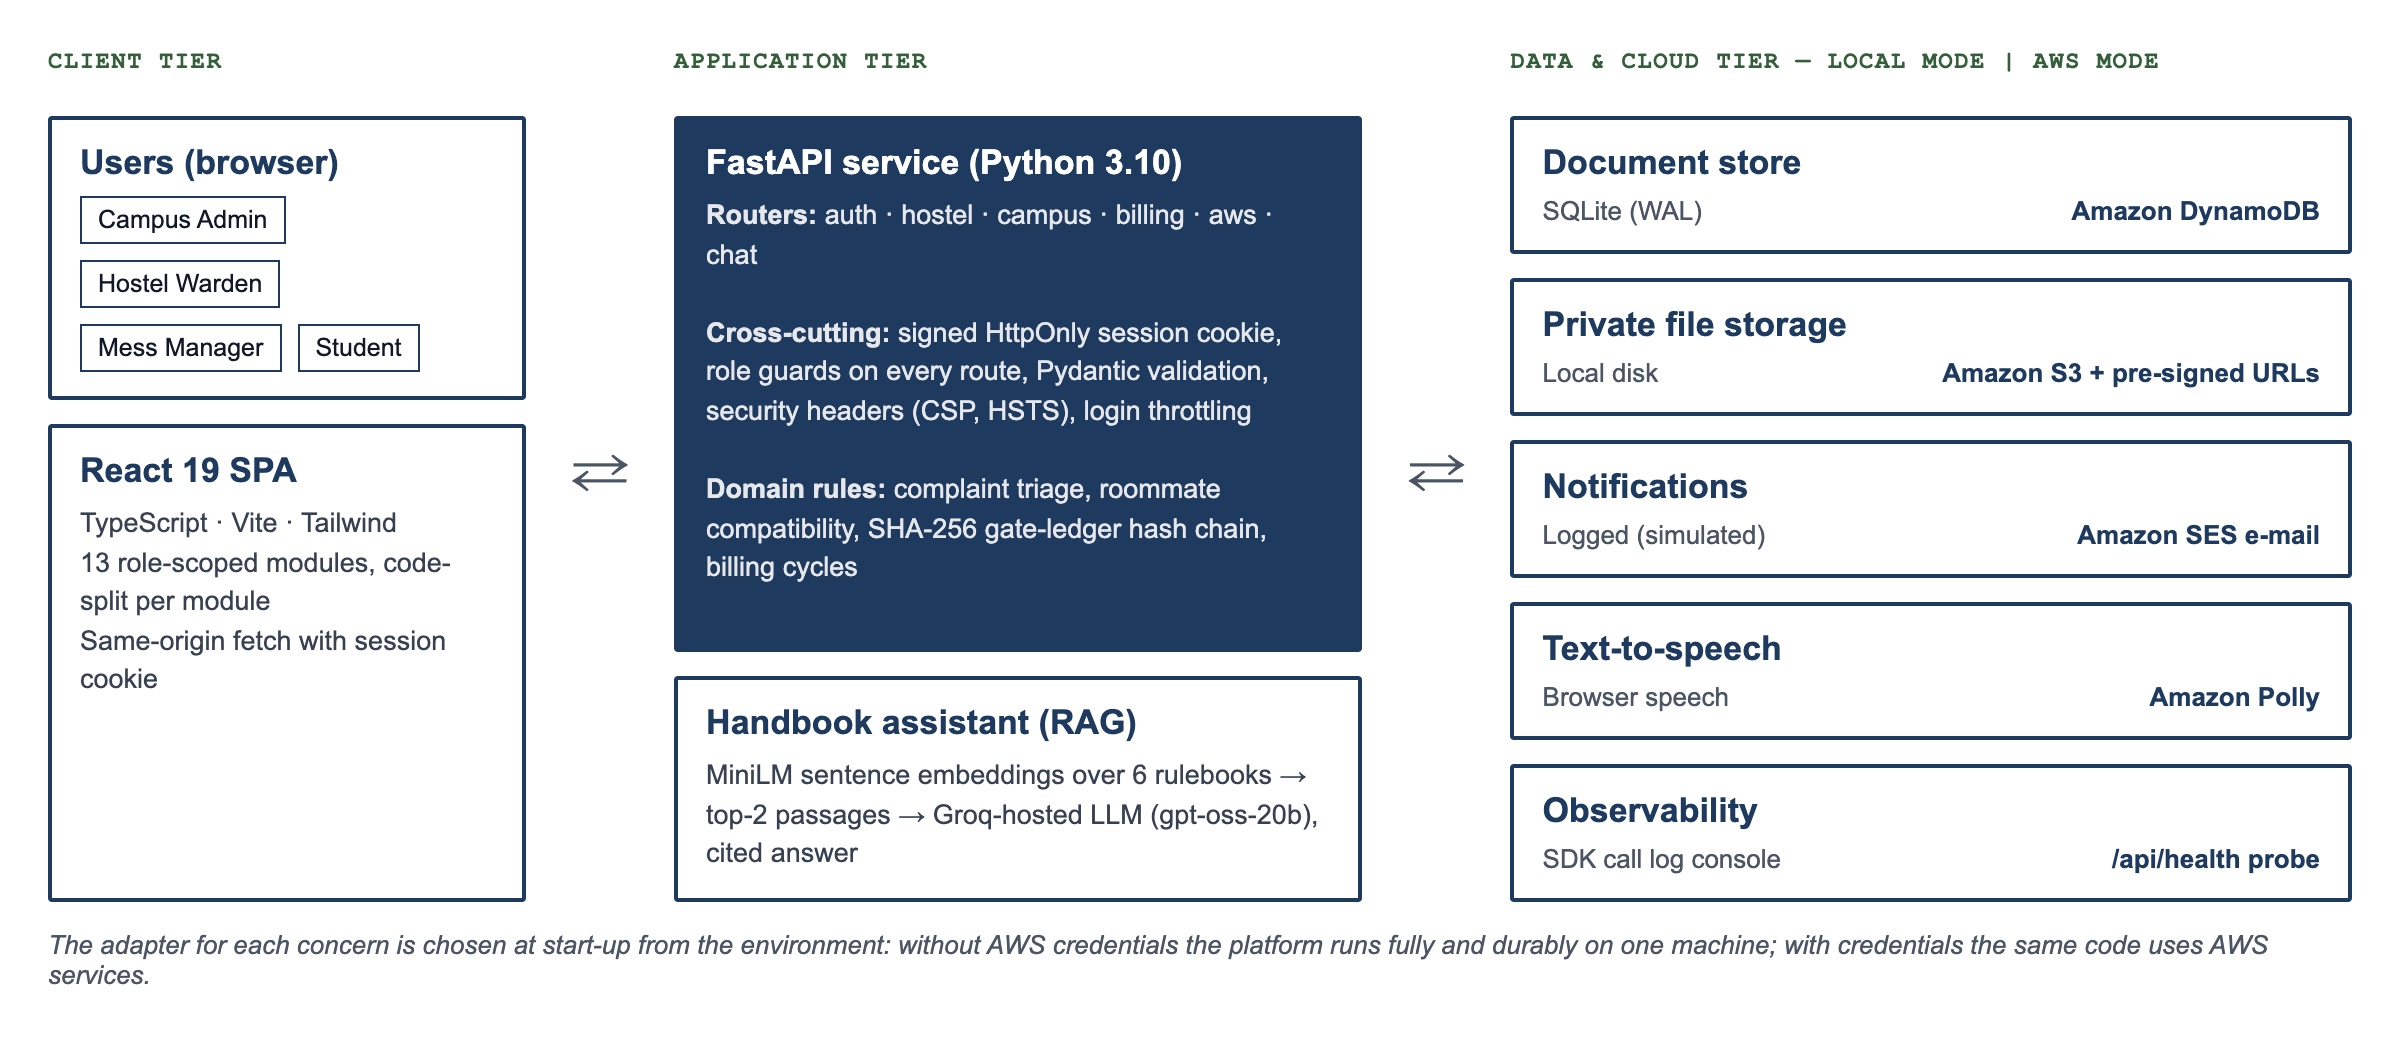
\includegraphics[width=\linewidth]{arch.png}
\caption{Three-tier architecture of Demeure AI with local and AWS adapters}\label{fig:arch}
\end{figure}

The data and cloud tier is selected at start-up. When AWS credentials are present the store uses DynamoDB (one table
per collection, created on demand with on-demand billing), uploads go to a private S3 bucket and are served through
five-minute pre-signed URLs, notifications are sent through SES and speech is synthesised by Polly. Without credentials
the same interfaces use SQLite in write-ahead-logging mode, the local disk, a logged e-mail simulation and the
browser's speech synthesis. Every call is written to an observable log that administrators can watch in the AWS
Console Hub.

\subsection{Role model and access control}
Authorisation is enforced on the server for every route; the user interface only hides what the server would refuse
anyway. Table~\ref{tab:roles} summarises which persona can use each module. Students can see only their own leaves,
visitors, surveys, complaints and grievances. Staff responses never reveal who filed an anonymous grievance.

\begin{table}[!htbp]\centering\small
\caption{Role-based access to modules}\label{tab:roles}
\begin{tabularx}{\linewidth}{L>{\centering\arraybackslash}p{0.82in}>{\centering\arraybackslash}p{0.82in}>{\centering\arraybackslash}p{0.82in}>{\centering\arraybackslash}p{0.95in}}
\toprule\head \textbf{Module} & \textbf{Campus Admin} & \textbf{Hostel Warden} & \textbf{Mess Manager} & \textbf{Student}\\\midrule
Overview telemetry and AI handbook assistant & Yes & Yes & Yes & Yes\\
Resident directory, onboarding and import & Yes & Yes & -- & Own record only\\
Academic hub, facilities and fleet, finance and campus life & Yes & -- & Finance only & Yes\\
Power grid diagnostics and billing dispatch & Yes & -- & -- & --\\
AWS Console Hub & Yes & -- & -- & --\\
Room allocation, survey responses, security gate, welfare & -- & Yes & -- & Survey form only\\
NLP complaint desk & Yes (manage) & Yes (manage) & -- & Yes (own tickets)\\
Mess and food optimiser & -- & -- & Yes (publish) & Yes (view, rate)\\
Student services: dues, payment, leave, visitor pass & -- & -- & -- & Yes\\
\bottomrule
\end{tabularx}
\end{table}

\subsection{Data model}
All records are JSON documents with a string identifier, stored in named collections (Table~\ref{tab:data}). The same
document shape is written to SQLite or DynamoDB; floating-point values are converted to DynamoDB decimals
transparently. Server-generated identifiers such as \texttt{L-3F9A2C} use a cryptographically random suffix, so IDs
cannot collide under concurrent requests.

\begin{table}[!htbp]\centering\small
\caption{Principal collections}\label{tab:data}
\begin{tabularx}{\linewidth}{P{1.55in}LP{1.85in}}
\toprule\head \textbf{Collection} & \textbf{Key fields} & \textbf{Written by}\\\midrule
students & regNo, name, gender, block, room, status, credential hash; \textit{encrypted:} phone, date of birth, blood group, guardian details, address, medical notes & Seed; staff onboarding and import\\
leaves & studentId, startDate, endDate, reason, proofUrl, status & Student (create), Warden (approve/deny)\\
visitors & hostId, visitor, date, purpose, status, passCode & Student (request), Warden (approve/deny)\\
billing / payments & powerRate, baseFee, cycleId / receiptId, amount, cycleId & Admin (dispatch) / Student (pay)\\
surveys & ownerId, lifestyle answers, preferred block and floor & Student (upsert); 100 seeded students\\
room\_allocations & occupants, maxOccupants & Warden\\
complaints, maintenance, bookings, grievances & text, category, priority, status, filedBy & All roles (create), staff (status)\\
mess\_menu, mess\_reviews & weekly days / rating, meal, suggestion & Mess Manager / Student\\
gate\_ledger & seq, time, subject, status, prevHash, hash & Warden (gate events)\\
files & key, ownerId, contentType & Upload endpoint\\
\bottomrule
\end{tabularx}
\end{table}

\subsection{Algorithms}\label{sec:algo}
\textbf{(a) Credential verification and sessions.} Staff PINs and student access codes are stored only as
PBKDF2-HMAC-SHA256 hashes with a random 16-byte salt and 120,000 iterations [10], and are compared in constant time.
After a successful login the server issues a token
\begin{equation}
t = \mathrm{B64}(p)\;\Vert\;\text{``.''}\;\Vert\;\mathrm{B64}\big(\mathrm{HMAC}_{\mathrm{SHA256}}(K,\ \mathrm{B64}(p))\big),
\end{equation}
where the payload $p$ holds the user identity, role and an expiry time and $K$ is the server's secret key [9]. The token
is set as an HttpOnly, SameSite=Strict cookie [11]. On each request the signature is recomputed and compared in
constant time; a modified payload (for example a forged role) or an expired token is rejected with HTTP 401. Ten failed
logins from one client within five minutes return HTTP 429.

\textbf{(b) Retrieval-augmented handbook assistant.} Each of the eight rulebooks is split into sections at level-two
headings and every section is prefixed with its rulebook's title, giving 30 chunks; each chunk is embedded with the
all-MiniLM-L6-v2 encoder [2], [3]. For a query $q$
the assistant computes the cosine similarity against every chunk $c$,
\begin{equation}
\mathrm{sim}(q, c) = \frac{\mathbf{e}_q \cdot \mathbf{e}_c}{\lVert \mathbf{e}_q \rVert\,\lVert \mathbf{e}_c \rVert},
\end{equation}
keeps up to three chunks with similarity above 0.2 that are within 0.12 of the best match, and passes them to
the language model with the instruction to answer only
from that context [1]. The answer is returned with the cited file names. If no model is configured, the retrieved
policy text is returned verbatim, so the feature degrades gracefully.

\textbf{(c) Roommate compatibility.} Each lifestyle dimension $d$ (sleep, study, cleanliness, social) is mapped to an
ordinal scale $\{0, 1, 2\}$. For the warden's requested profile $a$ and a resident's survey $b$, the score is
\begin{equation}
S(a, b) = 100 \times \frac{\sum_d w_d \left(1 - |a_d - b_d|/2\right)}{\sum_d w_d},
\end{equation}
with weights $w = (0.30, 0.25, 0.25, 0.20)$. Residents who prefer the same block receive a +5 bonus, capped at 100.
Blocks A and B are single-gender, so when the target block is A or B only residents who chose that block are eligible;
Block C, which is mixed, ranks all residents. The top three candidates are returned with their scores.

\textbf{(d) Complaint triage.} Each category (Electrical, Plumbing, Structural, IT/WiFi) has a keyword list. A keyword
counts as a hit only when it occurs at the start of a word, so ``lock'' does not match ``Block''. The category with the
most hits wins; ties go to the more safety-critical category, and with no hits the complaint is General/Low. If any
hazard term (socket, spark, shock, fire, smoke, gas, flood and similar) appears, the priority is raised to CRITICAL with
a two-hour response target.

\textbf{(e) Tamper-evident gate ledger.} Gate events form a hash chain. With $h_0 = 0^{64}$ and canonical JSON
$C(e)$ of the fields time, subject, type, purpose and status, each entry stores
\begin{equation}
h_i = \mathrm{SHA\text{-}256}\big(h_{i-1} \,\Vert\, C(e_i)\big)
\end{equation}
[6], [8]. Verification recomputes the chain on every read; editing, reordering or deleting any past entry changes all
later hashes, and the warden console shows an integrity failure.

\textbf{(f) Billing cycles and idempotent payment.} Every rate dispatch by the administrator creates a new cycle
identifier. The student's statement is computed on the server as base fee + metered kWh $\times$ rate + mess fines, so
the client cannot change the amount. A payment is stored under the key (student, cycle), which makes a second payment
in the same cycle impossible (HTTP 409) while a new cycle reopens the dues.

\textbf{(g) Field-level encryption of resident records.} Each personal field value $m$ of a resident record $r$ is
stored as
\begin{equation}
c = n \,\Vert\, \mathrm{AES\text{-}GCM}_K\big(n,\ m,\ A = r \,\Vert\, f\big),
\end{equation}
with a fresh 96-bit nonce $n$ and the record identifier and field name $f$ as associated data $A$ [28]. The 256-bit
key $K$ is read from \texttt{DATA\_ENCRYPTION\_KEY}, which production mode requires; in development it is derived
from the session secret with HKDF-SHA256 [29]. Because $A$ binds each ciphertext to its record and field, a value
copied into another record or field fails authentication instead of decrypting. Name, course and room stay in clear
so staff can search; the directory shows masked phone numbers, and every full decryption by staff is written to the
audit log.

\textbf{(h) Onboarding and bed assignment.} A new resident is placed by a deterministic search: floors are tried in
order of distance from the preferred floor, with the preferred room type first, skipping rooms under maintenance,
full rooms and rooms occupied by residents of another gender. Blocks A and B accept only men and women respectively;
Block C accepts both but never mixes genders within a room. The same routine placed the 100 seeded residents. Each
new resident receives an eight-character one-time access code drawn from 31 unambiguous characters (about 40 bits),
e-mailed to them and stored only as a PBKDF2 hash; staff can reset a code or deactivate an account, which blocks
sign-in immediately.

\subsection{Cross-role workflow}
Figure~\ref{fig:flow} traces the leave-approval workflow across the student, the API, the storage and notification
services and the warden. The other workflows (visitor passes, complaints, grievances, bookings) follow the same pattern:
create by one role, a validated state transition by another, and a notification.

\begin{figure}[!htbp]\centering
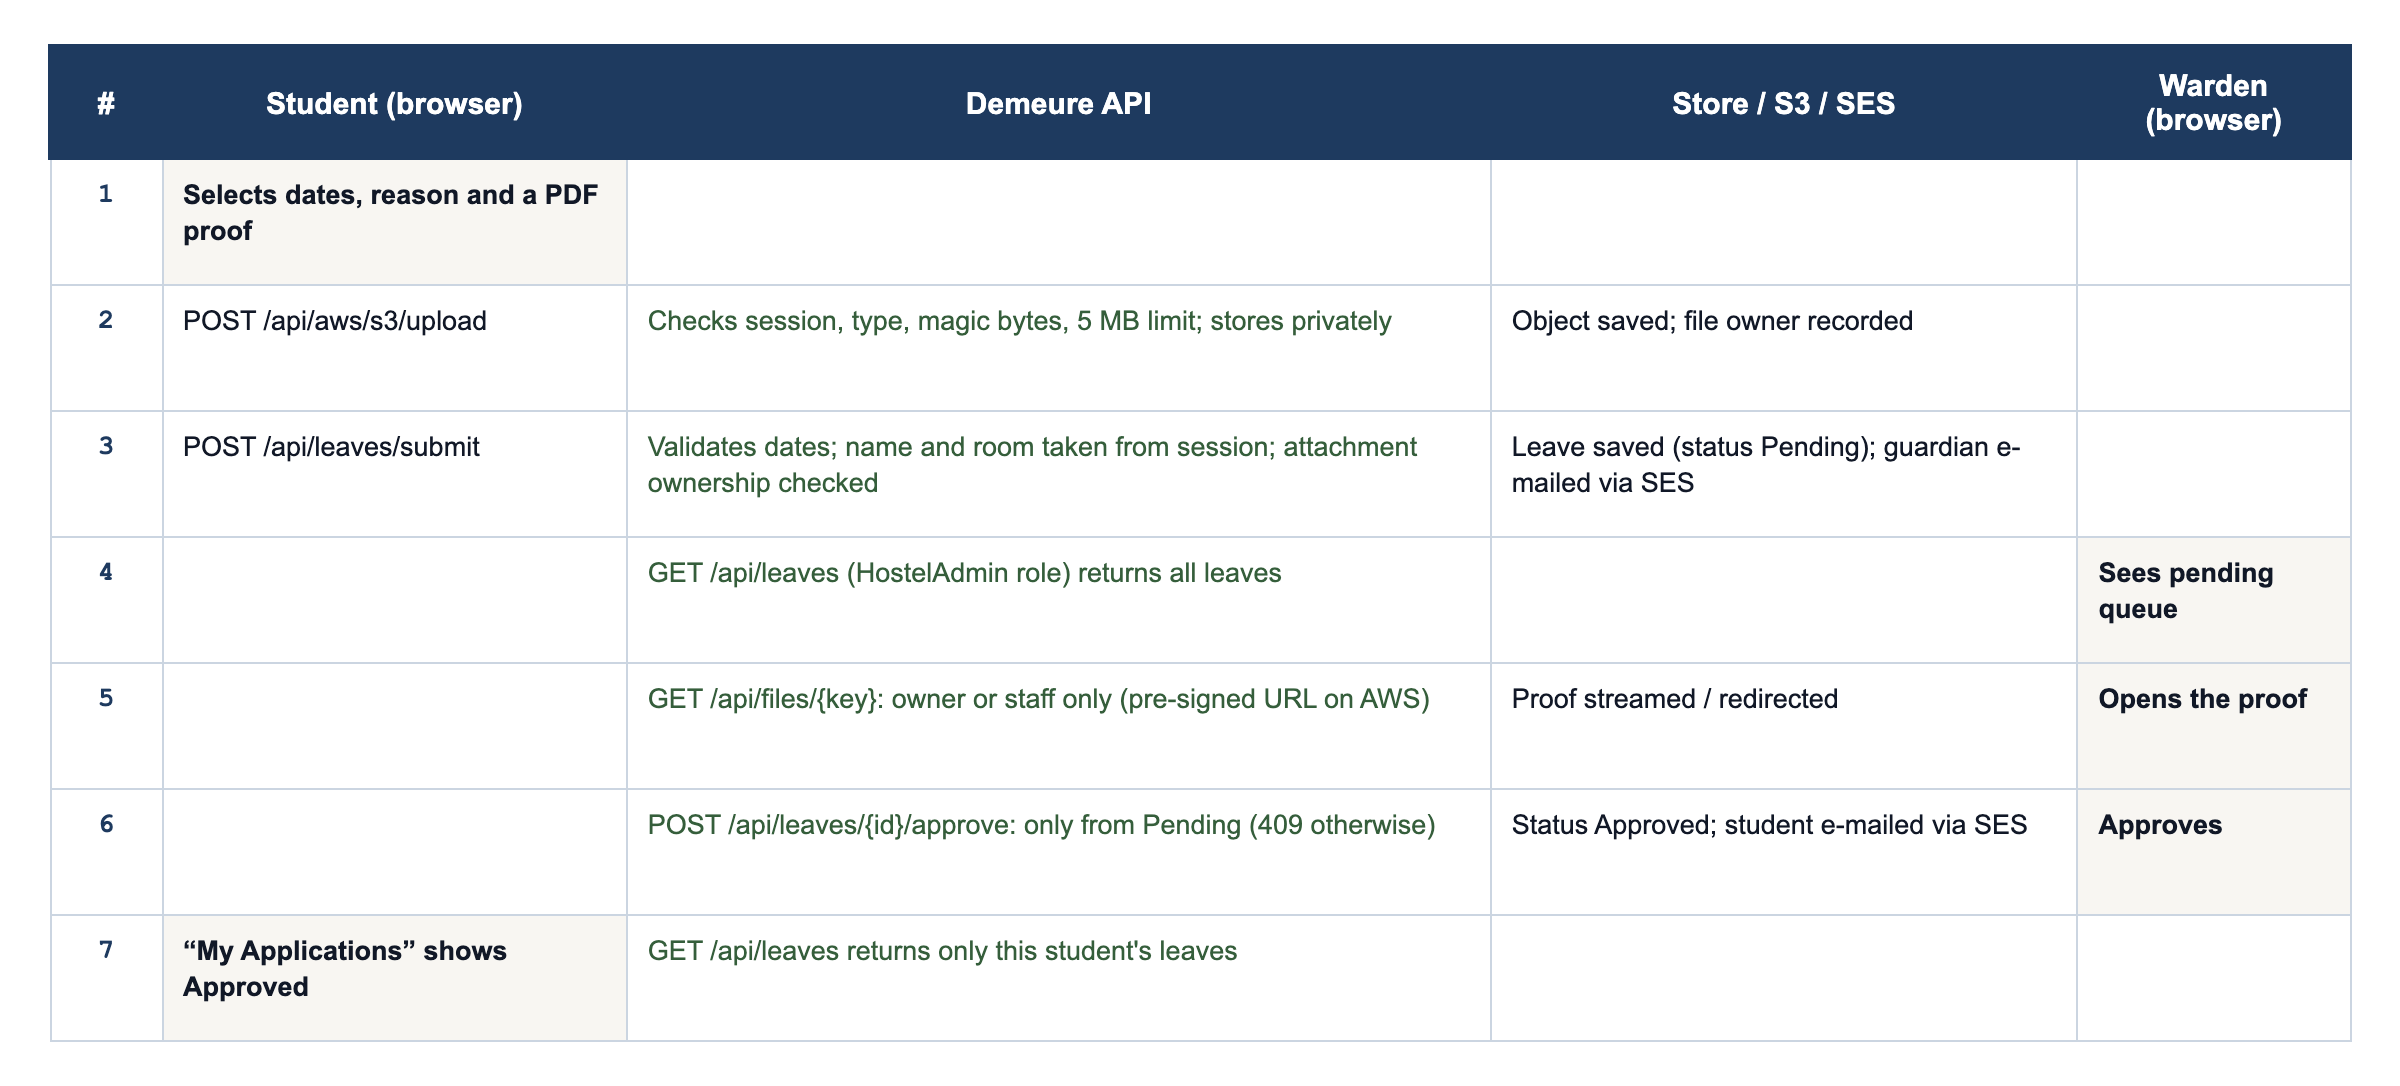
\includegraphics[width=0.95\linewidth]{flow.png}
\caption{Leave request with a private proof attachment, from submission to approval}\label{fig:flow}
\end{figure}

\section{Technical Descriptions}\label{sec:tech}
This section walks through the implemented modules using screenshots captured from the running application by an
automated Chrome session (Puppeteer) signed in as each persona. The complete source code is in the project repository;
key algorithms are reproduced in Appendix-1.

\subsection{Landing page and authentication}
The landing page (Fig.~\ref{fig:landing}) introduces the platform and leads to the persona picker
(Fig.~\ref{fig:roles}). Staff authenticate with a 12-digit PIN on an on-screen keypad and students with an institutional
e-mail and access code. Wrong credentials are rejected by the server. In production builds the demo hints are hidden,
and the server refuses to start with demo PINs or a weak signing key.

\begin{figure}[!htbp]\centering
\begin{subfigure}[b]{0.49\linewidth}\centering
  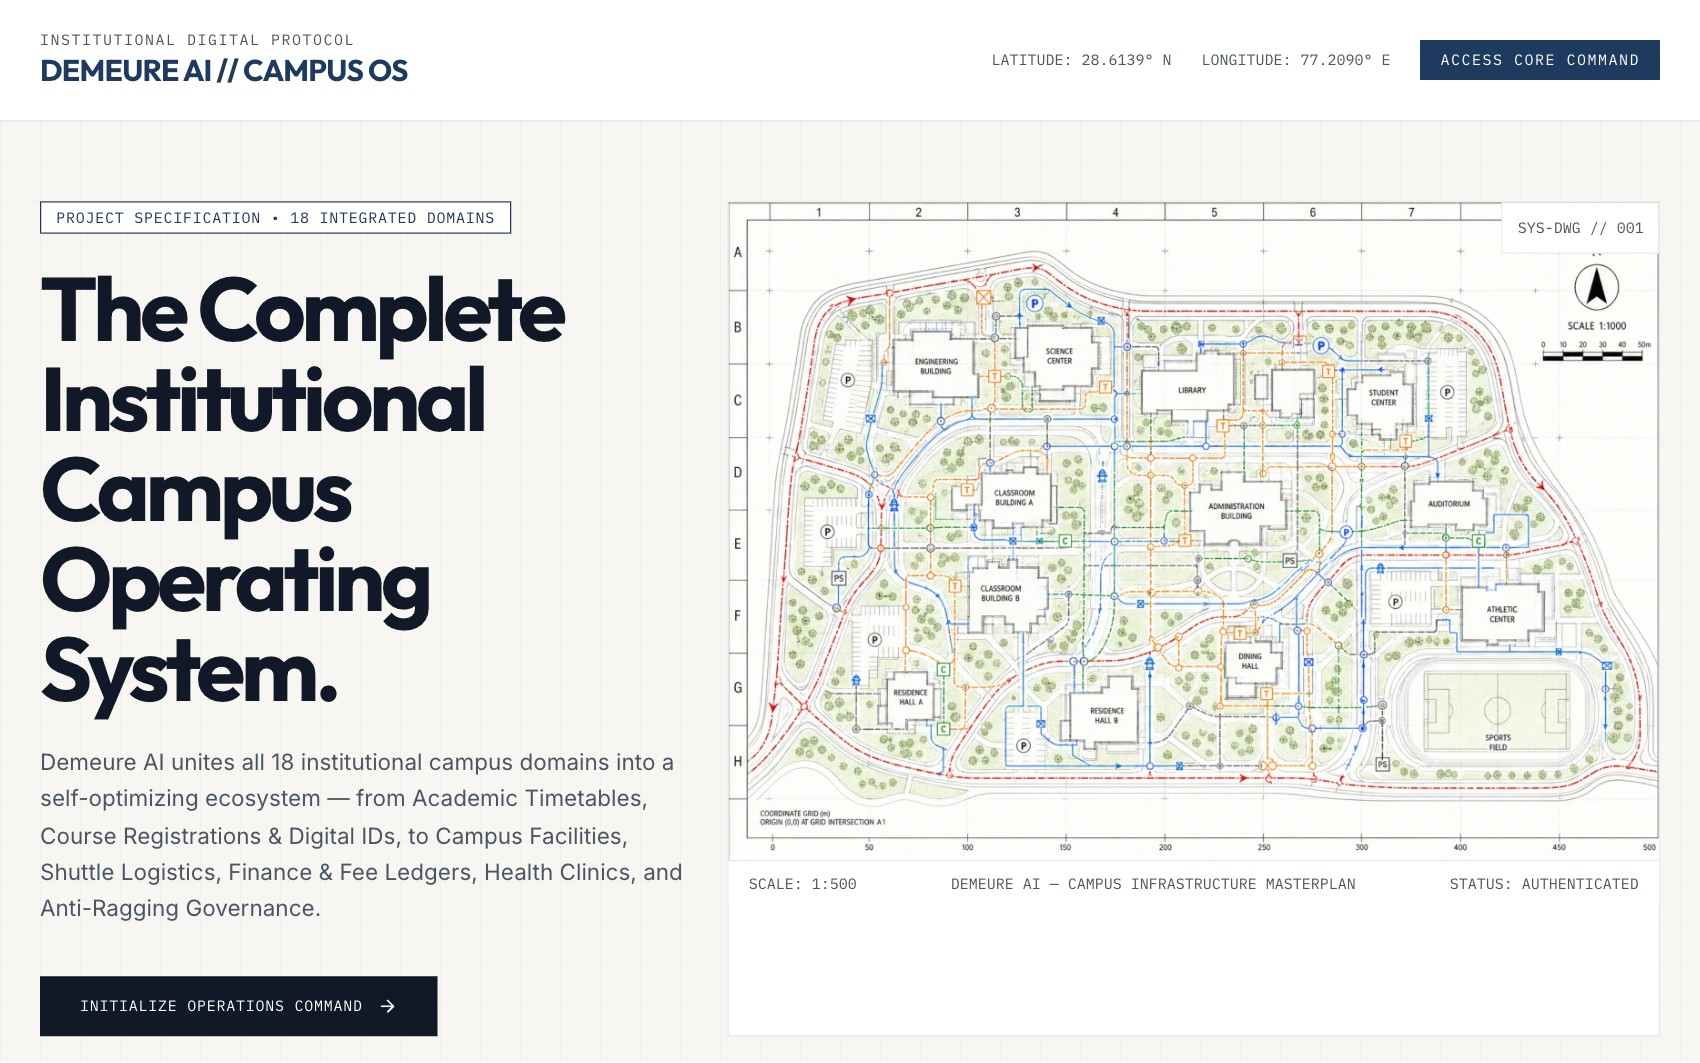
\includegraphics[width=\linewidth]{01-landing.jpg}\caption{Landing page}\label{fig:landing}
\end{subfigure}\hfill
\begin{subfigure}[b]{0.49\linewidth}\centering
  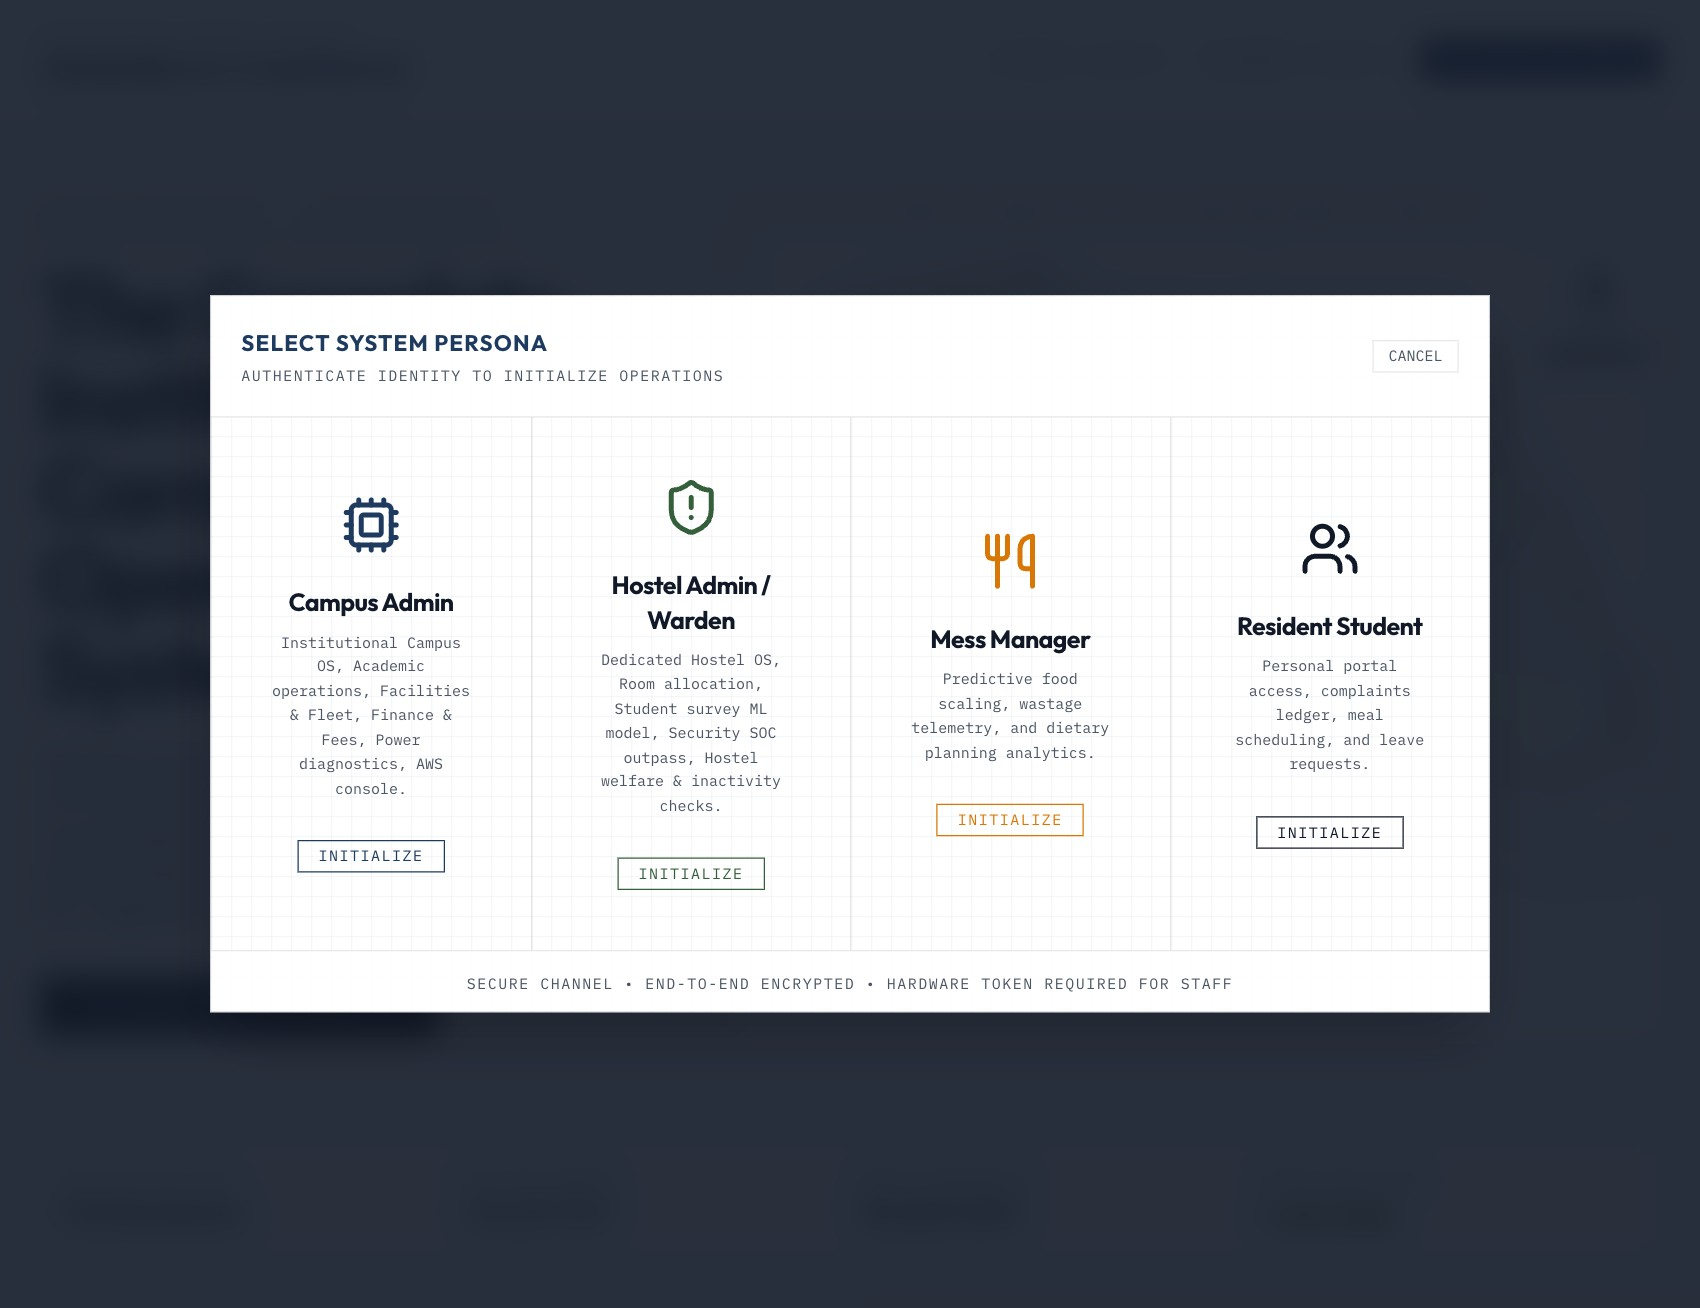
\includegraphics[width=\linewidth]{02-role-picker.jpg}\caption{Persona selection}\label{fig:roles}
\end{subfigure}
\caption{Entry to the platform}\label{fig:entry}
\end{figure}

\subsection{Student services: dues, payment, leave and visitor passes}
The student portal (Fig.~\ref{fig:portal}) shows the resident's own record and a server-computed statement for the current billing cycle and accepts a
UPI payment, after which a receipt is stored against the cycle (Fig.~\ref{fig:dues}). Leave applications validate dates
and accept a PDF, PNG or JPG proof of up to 5~MB, verified by its file signature and stored privately
(Fig.~\ref{fig:leaveform}). Students can also request visitor passes; on approval they receive a gate pass code
(Fig.~\ref{fig:visitor}).

\shot[0.36]{05-student-portal.jpg}{Student services portal with the resident's own record, decrypted for them\label{fig:portal}}

\begin{figure}[!htbp]\centering
\begin{subfigure}[b]{0.44\linewidth}\centering
  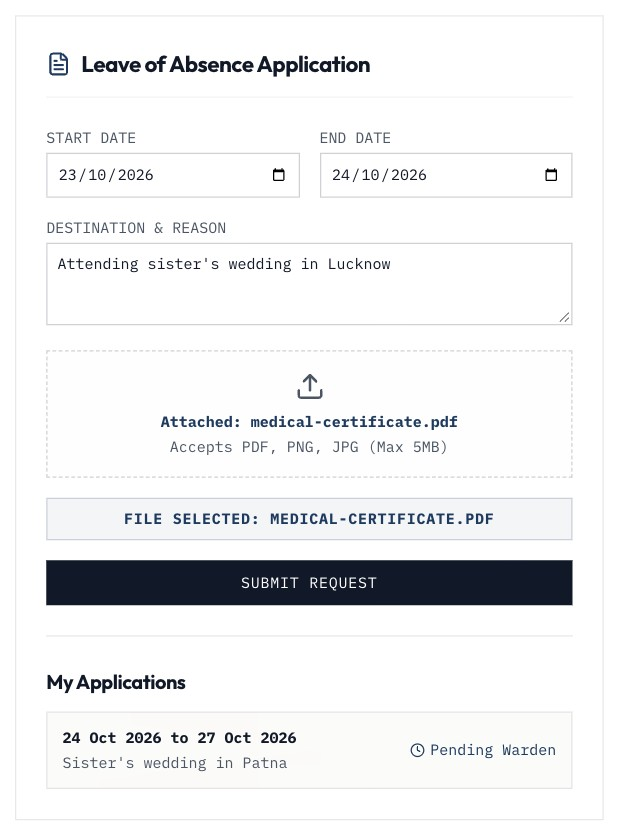
\includegraphics[height=3.5in]{f-leave-form.jpg}\caption{Leave application with proof attached}\label{fig:leaveform}
\end{subfigure}\hspace{0.04\linewidth}
\begin{subfigure}[b]{0.44\linewidth}\centering
  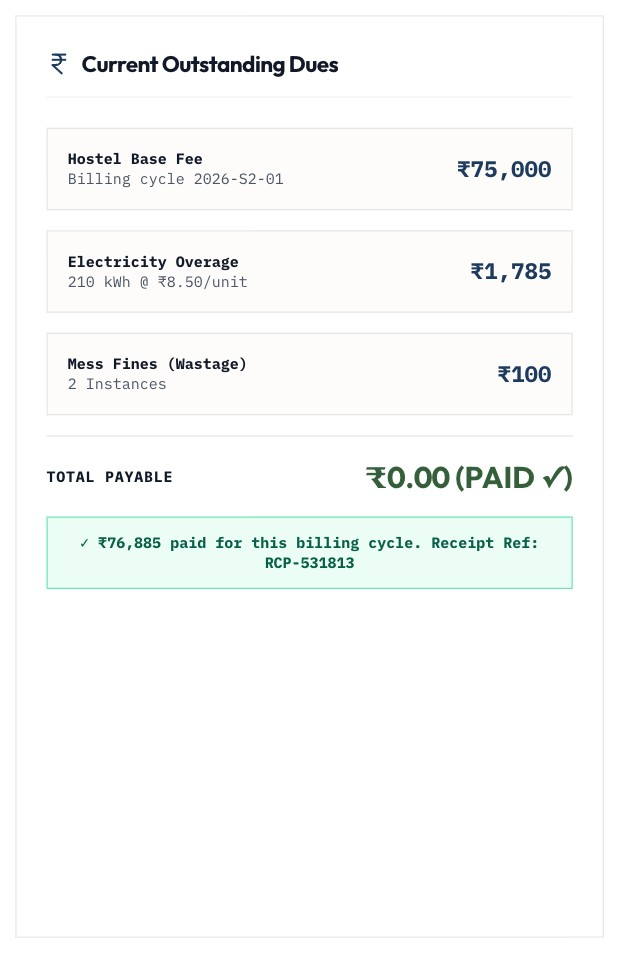
\includegraphics[height=3.5in]{f-dues-paid.jpg}\caption{Dues settled with a stored receipt}\label{fig:dues}
\end{subfigure}
\caption{Student self-service}\label{fig:student}
\end{figure}

\subsection{Hostel security operations}
The warden's security console lists pending leaves with a link to the private attachment (Fig.~\ref{fig:wleaves}) and
pending visitor requests. Approve and deny are one-way transitions; acting twice returns HTTP 409. The biometric gate
simulator writes entries to the hash-chained ledger, whose verification status is shown in the console
(Fig.~\ref{fig:ledger}).

\begin{figure}[!htbp]\centering
\begin{subfigure}[b]{0.485\linewidth}\centering
  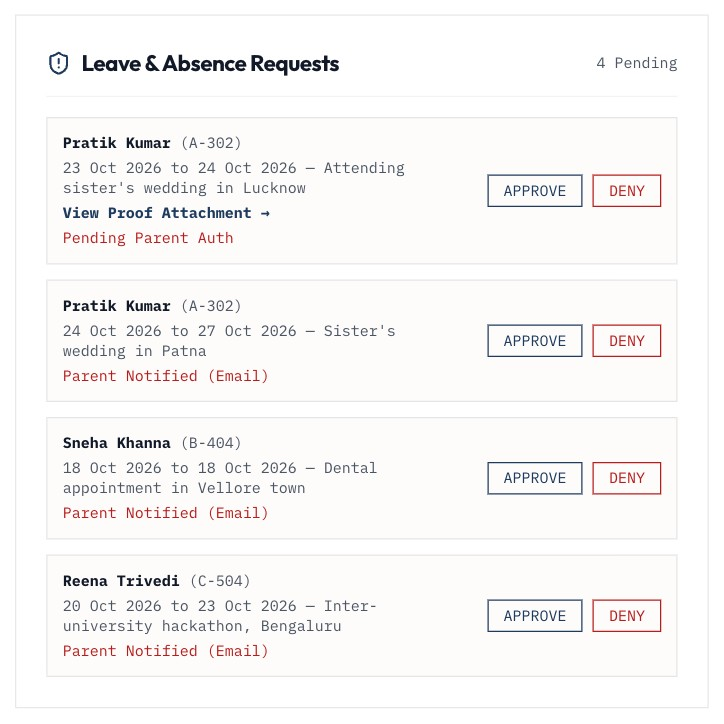
\includegraphics[width=\linewidth]{f-warden-leaves.jpg}\caption{Warden leave queue with proof attachment}\label{fig:wleaves}
\end{subfigure}\hfill
\begin{subfigure}[b]{0.485\linewidth}\centering
  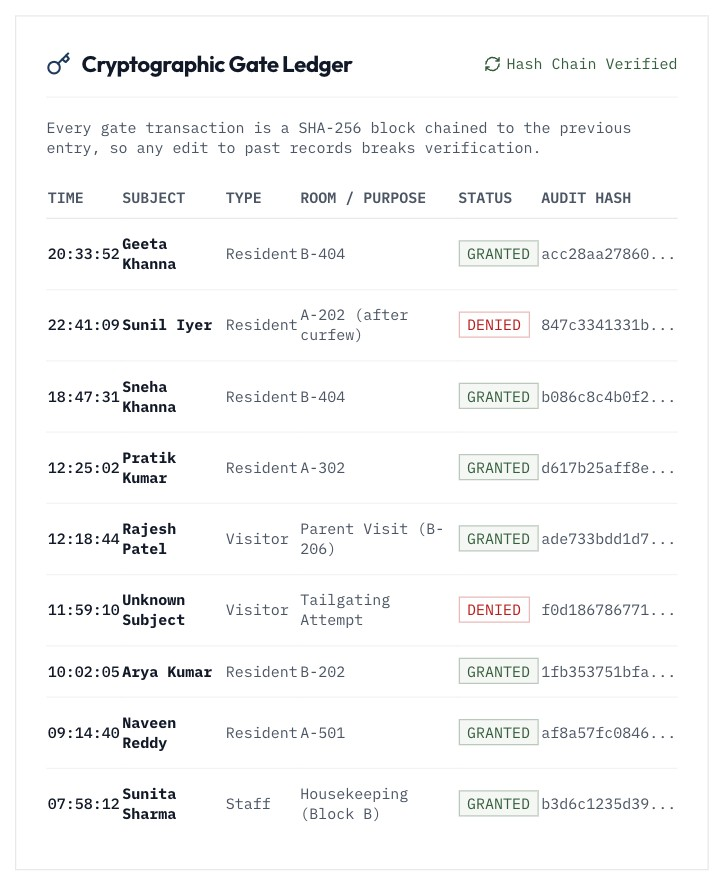
\includegraphics[width=\linewidth]{f-gate-ledger.jpg}\caption{Hash-chained gate ledger (chain verified)}\label{fig:ledger}
\end{subfigure}
\caption{Warden security console}\label{fig:security}
\end{figure}

\shot[0.3]{f-visitor-pass.jpg}{Visitor pass requests with issued gate pass codes\label{fig:visitor}}

\subsection{Survey and room allocation}
Students submit a room-preference survey that is saved on the server. Wardens see every response; the 100 seeded
responses plus new submissions feed the compatibility engine (Fig.~\ref{fig:survey}). Allocations are checked for
capacity and duplicates on the server and persisted, so every warden session sees the same occupancy.

\subsection{Resident directory and onboarding}
The Resident Directory (Fig.~\ref{fig:directory}) lists all residents with their programme, room, masked mobile
number and dues status for the current billing cycle. Selecting a resident decrypts the full profile for that
session and records the access in the audit log; the campus administrator can also display the record exactly as
stored, showing that personal fields are ciphertext (Fig.~\ref{fig:stored}). Staff register a resident through a
validated form (Fig.~\ref{fig:addres}): the server normalises phone numbers and blood groups, enforces the
single-gender block rules, assigns a bed and returns a one-time access code that is also e-mailed to the resident.
Batches are imported from a CSV or Excel sheet that is parsed in the browser; common header names are recognised,
valid rows are registered, and rows with errors are reported without stopping the import (Fig.~\ref{fig:import}).

\shot[0.31]{n-directory.jpg}{Resident Directory with a decrypted profile; access is audited\label{fig:directory}}

\begin{figure}[!htbp]\centering
\begin{subfigure}[b]{0.58\linewidth}\centering
  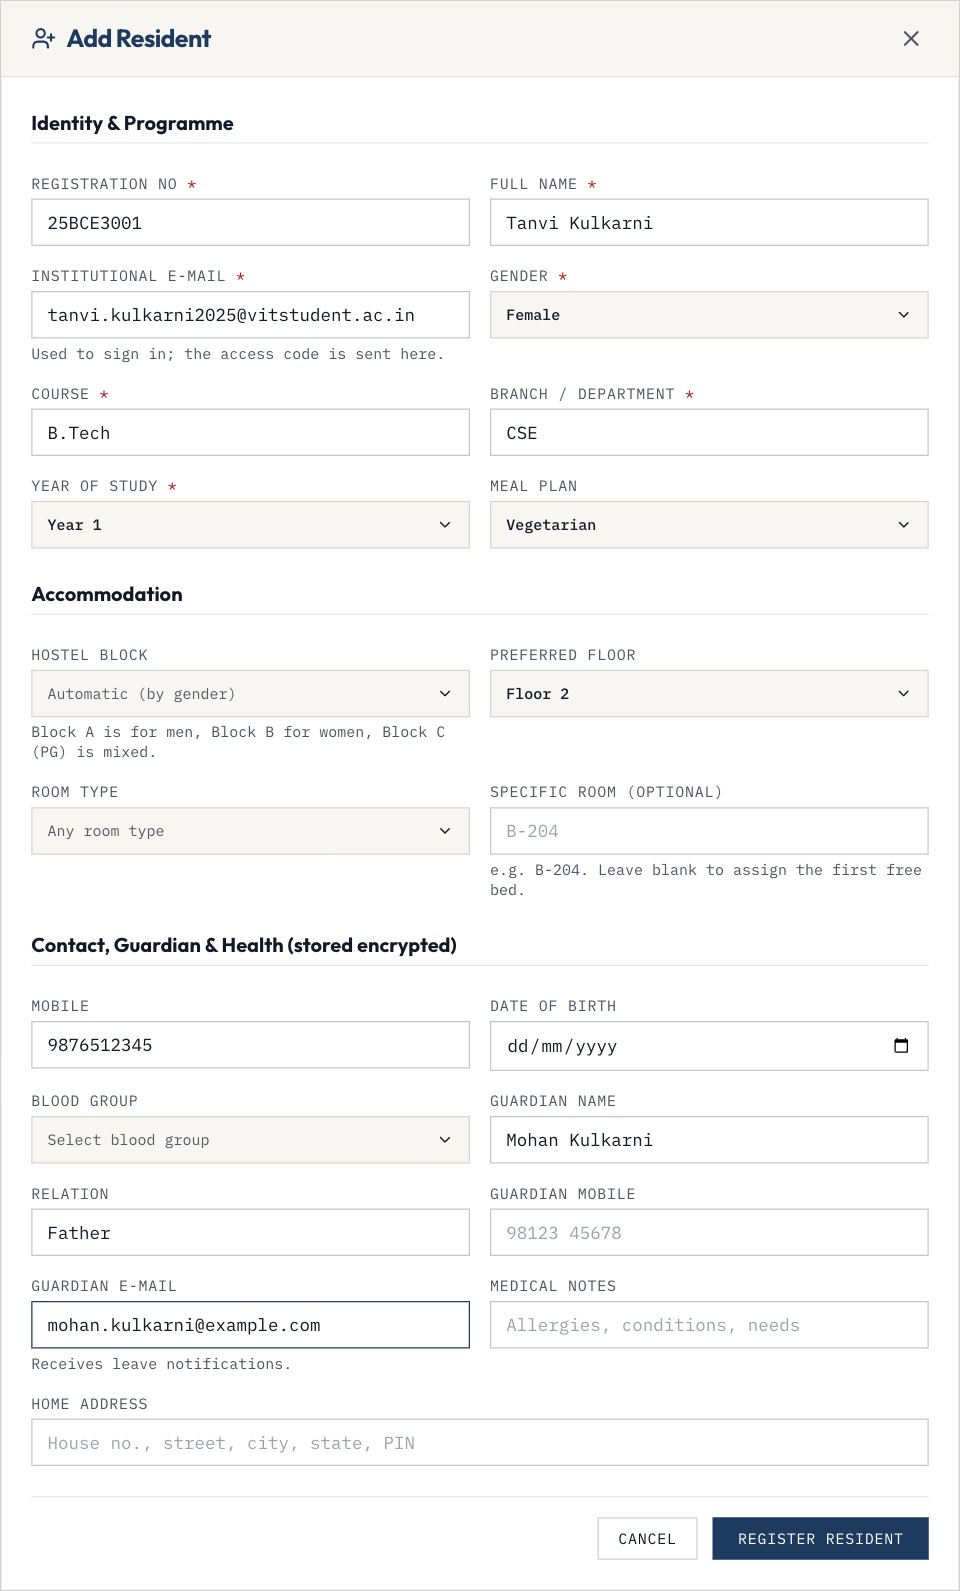
\includegraphics[height=3.6in]{n-add-resident.jpg}\caption{Validated registration form}\label{fig:addres}
\end{subfigure}\hspace{0.03\linewidth}
\begin{subfigure}[b]{0.34\linewidth}\centering
  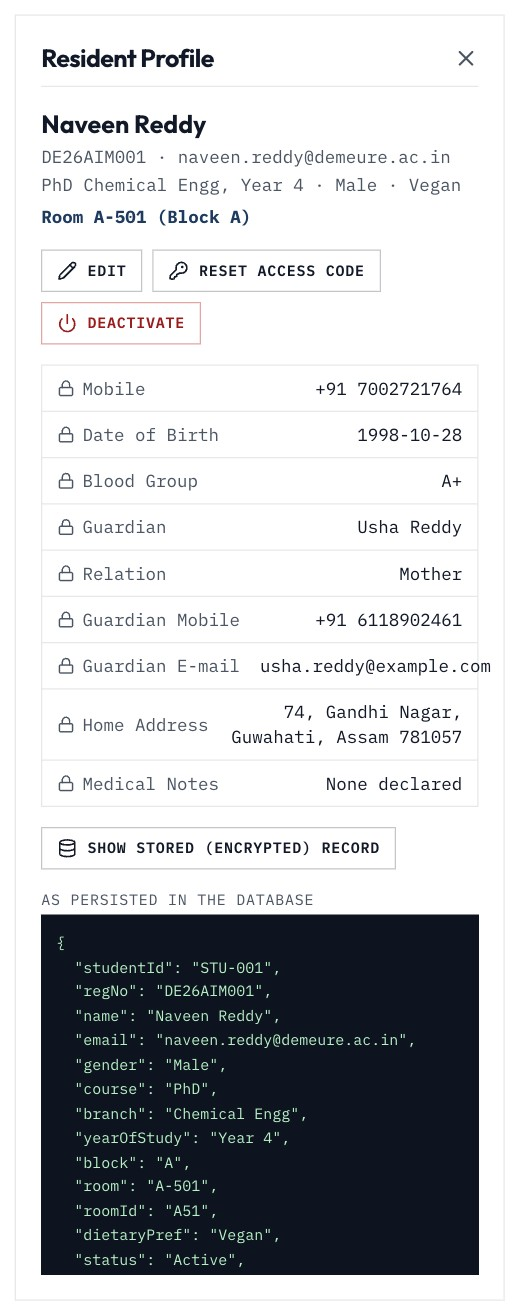
\includegraphics[height=3.6in]{n-stored-record.jpg}\caption{Record as stored (ciphertext)}\label{fig:stored}
\end{subfigure}
\caption{Onboarding and encryption at rest}\label{fig:onboarding}
\end{figure}

\shot[0.22]{n-import-result.jpg}{Spreadsheet import: valid rows registered with access codes, invalid row reported\label{fig:import}}

\shot[0.29]{22-survey-responses.jpg}{Survey responses and ML feature feed (101 responses)\label{fig:survey}}

\subsection{Decision-support engines}
The compatibility scorer ranks candidate roommates by the weighted score of Section~\ref{sec:algo}(c)
(Fig.~\ref{fig:compat}). On the complaint desk, a student describes a problem in free text and the triage engine
predicts its category, priority and response target before the ticket is logged (Fig.~\ref{fig:triage}); staff then
move tickets from Open to Dispatched to Resolved. The handbook assistant answers policy questions with citations to the
source rulebook (Fig.~\ref{fig:assistant}), and a speaker button reads the answer aloud through Amazon Polly or the
browser's speech synthesis.

\begin{figure}[!htbp]\centering
\begin{subfigure}[b]{0.4\linewidth}\centering
  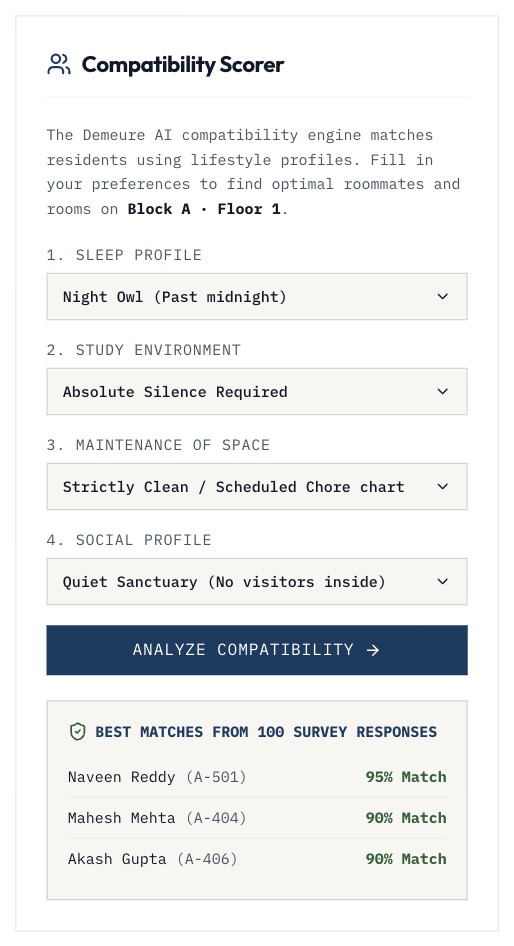
\includegraphics[height=3.4in]{f-compat.jpg}\caption{Compatibility scorer with ranked matches}\label{fig:compat}
\end{subfigure}\hspace{0.03\linewidth}
\begin{subfigure}[b]{0.55\linewidth}\centering
  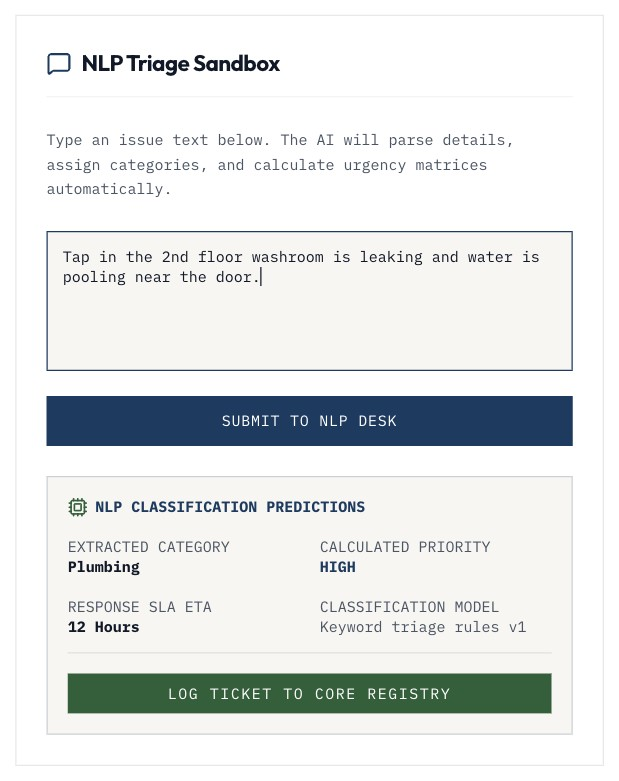
\includegraphics[height=3.4in]{f-triage.jpg}\caption{Complaint triage prediction}\label{fig:triage}
\end{subfigure}
\caption{Decision-support engines}\label{fig:engines}
\end{figure}

\shot[0.32]{29-ai-assistant.jpg}{Retrieval-augmented handbook assistant with citations\label{fig:assistant}}

\subsection{Mess, grievances and administration}
The mess manager uploads the weekly menu as an Excel sheet; it is validated and published to all students
(Fig.~\ref{fig:mess}), and student ratings appear in the manager's feedback feed. The grievance desk accepts anonymous
anti-ragging reports that staff can escalate without seeing the filer (Fig.~\ref{fig:grievance}). The power monitor
lets the administrator inspect per-zone load and dispatch a new billing cycle (Fig.~\ref{fig:power}), and the AWS
Console Hub shows service status and a live log of every data write, e-mail and upload (Fig.~\ref{fig:awslog}).

\begin{figure}[!htbp]\centering
\begin{subfigure}[b]{0.485\linewidth}\centering
  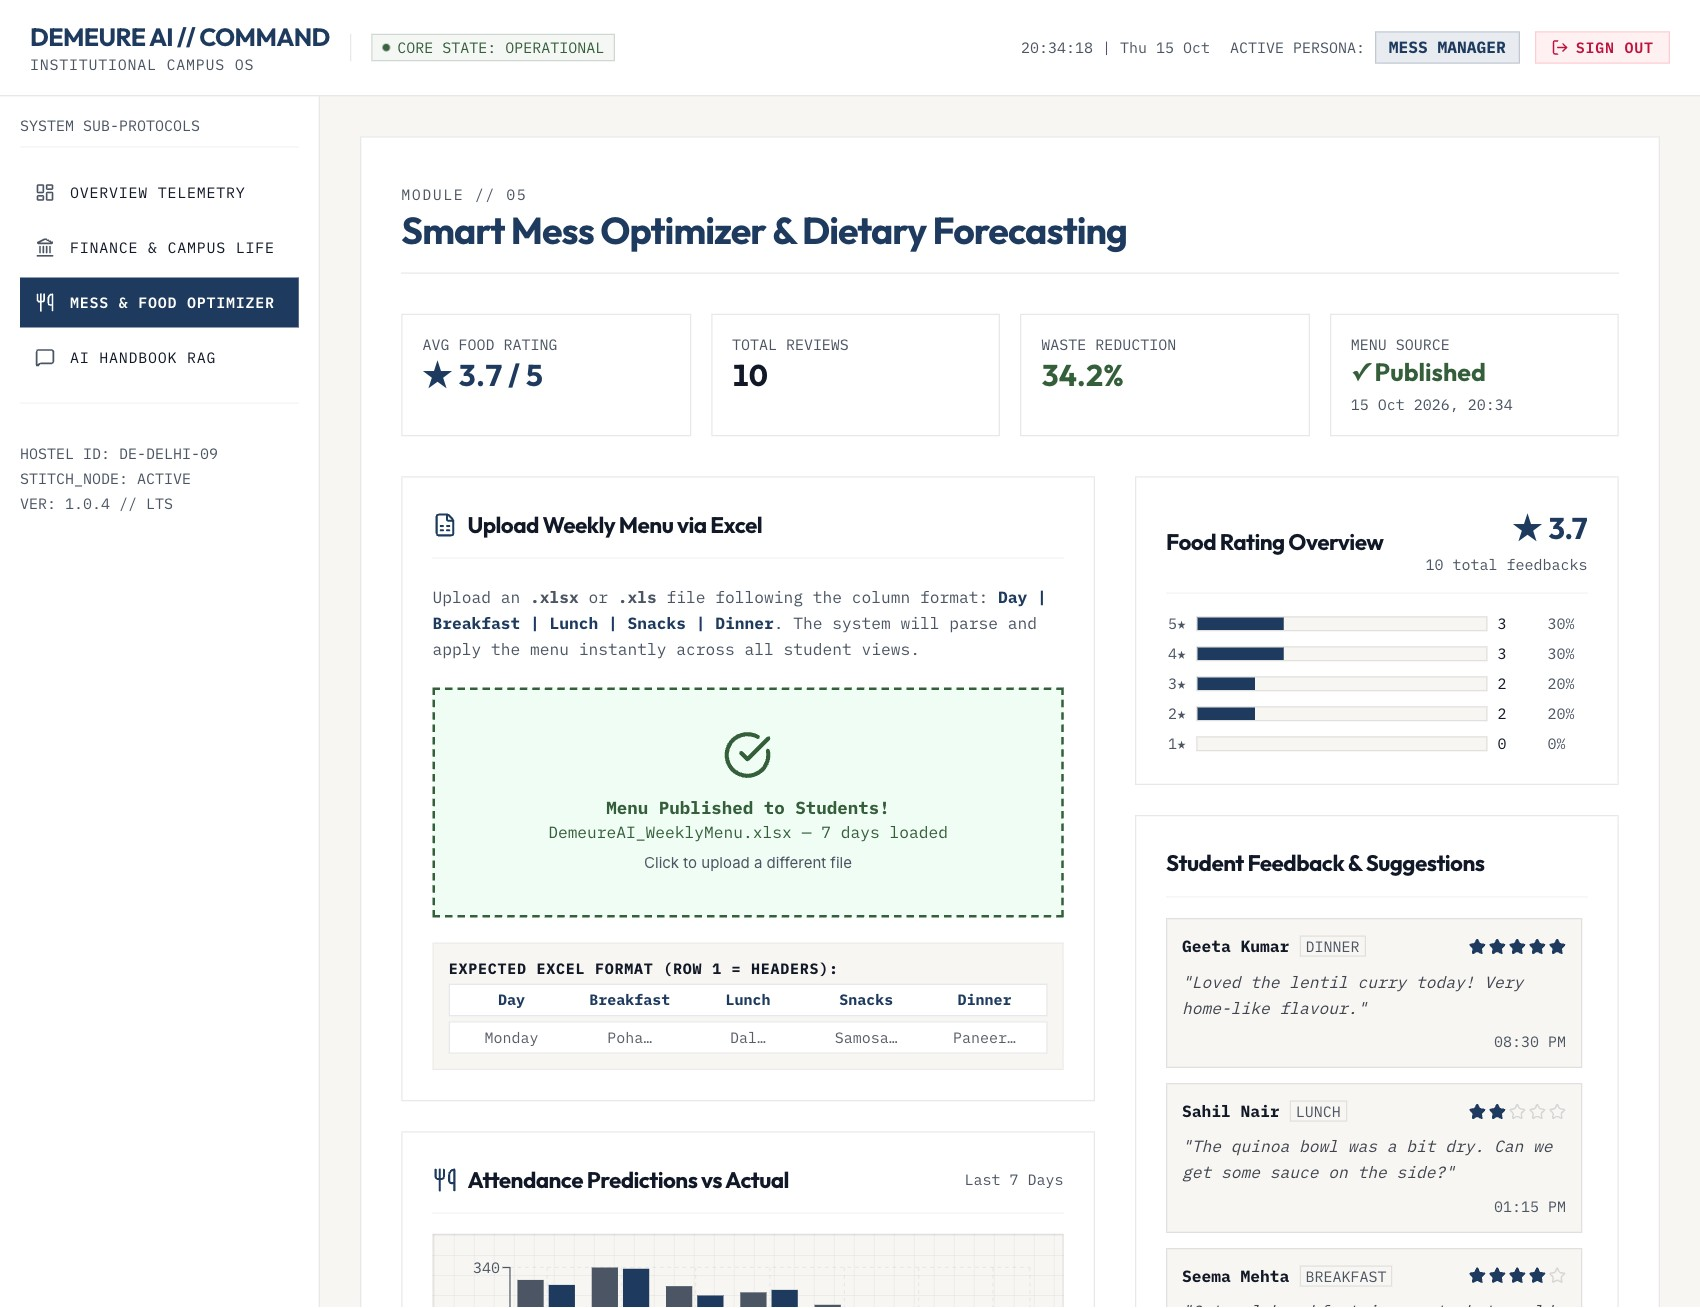
\includegraphics[width=\linewidth]{30-mess-manager-upload.jpg}\caption{Weekly menu published from Excel}\label{fig:mess}
\end{subfigure}\hfill
\begin{subfigure}[b]{0.485\linewidth}\centering
  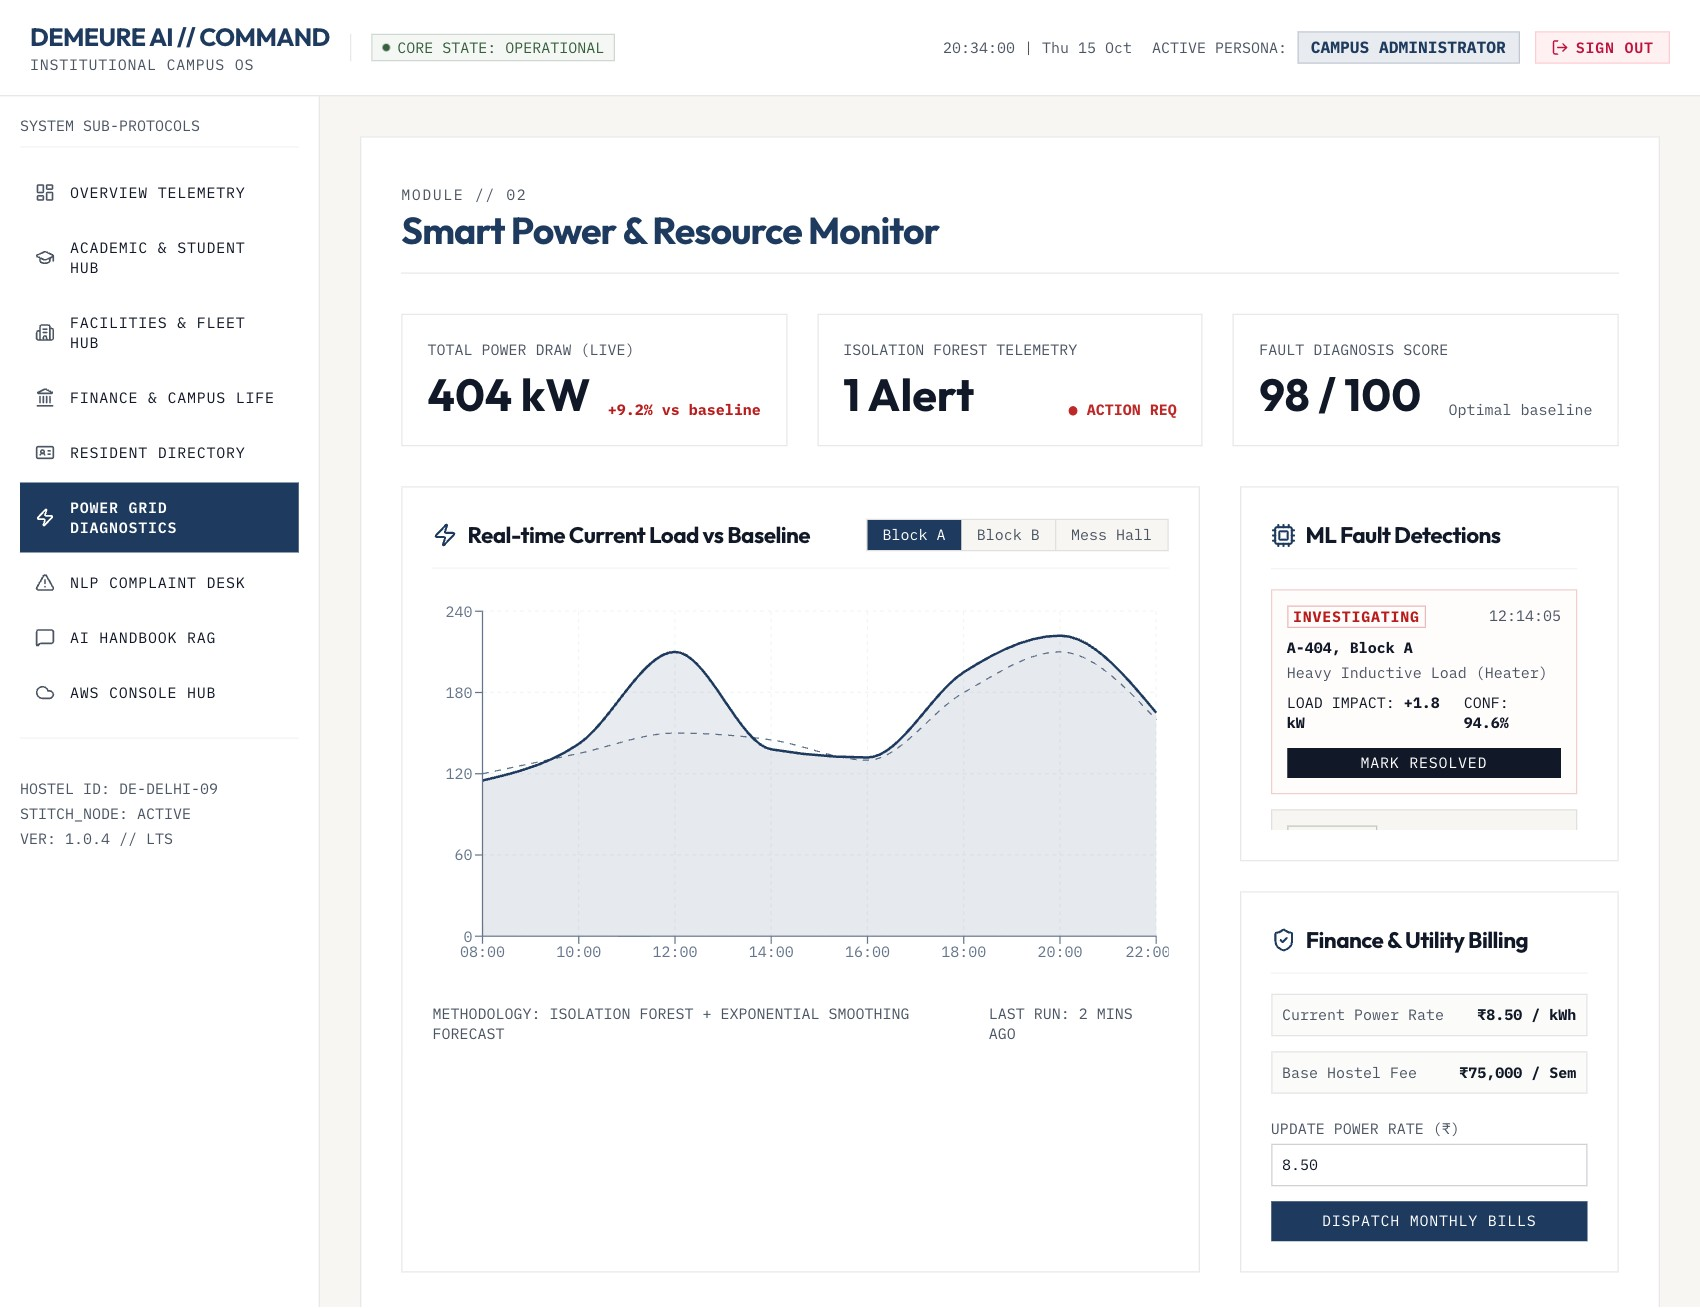
\includegraphics[width=\linewidth]{16-admin-power-billing.jpg}\caption{Power monitor and billing-cycle dispatch}\label{fig:power}
\end{subfigure}
\caption{Mess manager and campus administrator workspaces}\label{fig:admin}
\end{figure}

\shot[0.25]{f-grievance-admin.jpg}{Anonymous grievances triaged by staff\label{fig:grievance}}
\shot[0.2]{f-aws-logs.jpg}{AWS SDK call log console\label{fig:awslog}}

\subsection{Application programming interface}
Table~\ref{tab:api} lists representative endpoints. All request bodies are validated with Pydantic models; validation
errors return HTTP 422 with a readable message. Unknown \texttt{/api} paths return a JSON 404 instead of the web page.

\begin{table}[!htbp]\centering\small
\caption{Representative REST endpoints}\label{tab:api}
\begin{tabularx}{\linewidth}{>{\raggedright\arraybackslash\ttfamily}p{2.85in}P{1.2in}L}
\toprule\head \normalfont\textbf{Endpoint} & \textbf{Role} & \textbf{Purpose}\\\midrule
POST /api/auth/login, /logout; GET /api/auth/session & Public & Sign in, sign out, restore session\\
POST /api/aws/s3/upload; GET /api/files/\{key\} & Signed in & Private upload; owner or staff download\\
GET /api/billing/statement; POST /api/payments & Student & Server-computed dues; UPI payment\\
POST /api/billing/update & Campus Admin & Dispatch a new billing cycle\\
POST /api/leaves/submit; /api/leaves/\{id\}/approve|deny & Student / Warden & Leave workflow\\
POST /api/visitors; /api/visitors/\{id\}/approve|deny & Student / Warden & Visitor pass workflow\\
PUT /api/surveys/me; POST /api/rooms/compatibility & Student / Warden & Survey upsert; roommate ranking\\
POST /api/rooms/\{room\}/allocate & Warden & Capacity-checked allocation\\
POST /api/complaints/classify, /api/complaints & Signed in & Triage preview; file complaint\\
GET /api/gate/ledger; POST /api/gate/events & Warden & Hash-chained gate log\\
GET /api/students; GET /api/students/\{id\} & Staff & Directory (masked); decrypted profile (audited)\\
POST /api/students; POST /api/students/import & Staff & Register one resident; spreadsheet import\\
PATCH /api/students/\{id\}; POST .../reset-code & Staff & Edit, move, deactivate; new access code\\
GET /api/students/me & Student & Own decrypted record\\
PUT /api/mess/menu; POST /api/mess/reviews & Mess Manager / Student & Publish menu; rate meals\\
POST /api/chat/query & Signed in & Handbook assistant\\
GET /api/health & Public & Liveness and readiness probe\\
\bottomrule
\end{tabularx}
\end{table}

\subsection{Deployment}
A two-stage Dockerfile builds the React application with Node 22 and runs it, together with the API, in a Python 3.10
slim image as an unprivileged user. CPU-only PyTorch keeps the image small, and the embedding model is downloaded during
the build so containers start without network access. A HEALTHCHECK polls \texttt{/api/health}, data is kept on a named
volume, and \texttt{docker compose} starts the service in one command. In production mode the
service refuses to start without a strong signing key, an encryption key and non-demo PINs, sends
Content-Security-Policy, HSTS and frame-deny headers and disables the interactive API documentation. A GitHub Actions
workflow runs lint, the production build, a dependency audit and the backend tests on every push.

% ================================================================== 4
\chapter{HARDWARE/SOFTWARE TOOLS USED}
The project is entirely software-based. Table~\ref{tab:hw} lists the hardware used for development and the recommended
deployment target; Table~\ref{tab:sw} lists the software stack with the exact versions pinned in the repository.

\begin{table}[!htbp]\centering\small
\caption{Hardware}\label{tab:hw}
\begin{tabularx}{\linewidth}{P{1.55in}LP{2.0in}}
\toprule\head \textbf{Item} & \textbf{Specification} & \textbf{Use}\\\midrule
Development machine & Apple M4, 16 GB RAM, macOS 26.6 & Coding, testing, model inference, screenshots\\
Deployment target (recommended) & 1 vCPU / 2 GB RAM Linux VM, e.g.\ AWS EC2 t3.small, 20 GB disk & Single-container production deployment\\
Client devices & Any modern browser on laptop or phone & Use by all four personas\\
\bottomrule
\end{tabularx}
\end{table}

\begin{table}[!htbp]\centering\small
\caption{Software tools and libraries}\label{tab:sw}
\begin{tabularx}{\linewidth}{P{0.75in}LP{2.05in}}
\toprule\head \textbf{Layer} & \textbf{Tool / library (version)} & \textbf{Purpose}\\\midrule
Frontend & React 19.2, TypeScript 6.0, Vite 8.0 & Single-page application and build\\
  & Tailwind CSS 3.4, Lucide icons, Recharts 3.8; IBM Plex Mono, Inter and Outfit fonts & Styling, icons, charts, typography\\
 & SheetJS xlsx 0.20.3 & Excel import/export (menu, survey export)\\
Backend & Python 3.10, FastAPI 0.136, Uvicorn 0.49, Pydantic 2.13 & REST API, validation, ASGI server\\
 & SQLite (Python standard library) & Local document store\\
AI / ML & sentence-transformers 5.5 (all-MiniLM-L6-v2), NumPy 2.2 & Embeddings and similarity search\\
 & Groq API (openai/gpt-oss-20b); Google Gemini (optional fallback) & Grounded answer generation\\
Cloud & boto3 1.43: Amazon DynamoDB, S3, SES, Polly & Managed storage, files, e-mail, speech\\
Security & cryptography 49.0 (AES-256-GCM, HKDF) & Field-level encryption of personal data\\
Testing & pytest 8.4, HTTPX 0.28, Puppeteer (headless Chrome) & API tests, end-to-end scenarios, readability audit\\
Quality & ESLint 10 with React Hooks rules, npm audit & Static analysis and dependency audit\\
DevOps & Docker, Docker Compose, GitHub Actions & Container image, deployment, CI\\
Design & Figma (wireframes) & UI wireframes for nine modules\\
\bottomrule
\end{tabularx}
\end{table}

% ================================================================== 5
\chapter{RESULT ANALYSIS}
The implemented system was evaluated on functional correctness, security behaviour, performance and the quality of its
three intelligent components. All measurements in this chapter were taken on the development machine of
Table~\ref{tab:hw} against the running application.

\section{Functional verification}
Fourteen cross-role scenarios, made up of 57 individual checks, were scripted in headless Chrome
(Table~\ref{tab:e2e}). Each scenario signs in the relevant
personas in separate browser contexts, performs the workflow through the user interface and checks that the other role
sees the result. All passed from a freshly seeded database with no browser console errors and no failed API calls
other than the deliberate negative checks (a wrong access code and a deactivated account).

\begin{table}[!htbp]\centering\small
\caption{End-to-end scenario results}\label{tab:e2e}
\begin{tabularx}{\linewidth}{>{\centering\arraybackslash}p{0.25in}LP{1.45in}>{\centering\arraybackslash}p{0.45in}}
\toprule\head \textbf{\#} & \textbf{Scenario} & \textbf{Roles} & \textbf{Result}\\\midrule
1 & Leave request with PDF proof; warden opens the private file and approves & Student, Warden & Pass\\
2 & Visitor pass request; approval issues a gate pass code & Student, Warden & Pass\\
3 & Billing-cycle dispatch; student pays server-computed dues; receipt stored & Admin, Student & Pass\\
4 & Survey submission joins 100 seeded responses; ranking; capacity-checked allocation & Student, Warden & Pass\\
5 & Complaint triage and status workflow (Open, Dispatched, Resolved) & Student, Warden & Pass\\
6 & Handbook question answered with citations & Student & Pass\\
7 & Weekly menu published from Excel; student rating reaches the manager & Mess Manager, Student & Pass\\
8 & Anonymous grievance escalated without exposing the filer & Student, Admin & Pass\\
9 & Facility booking approval and maintenance work-order progression & Student, Admin & Pass\\
10 & Biometric gate events appended to the verified hash chain & Warden & Pass\\
11 & Staff open an encrypted resident profile; the decryption appears in the audit log & Warden, Admin & Pass\\
12 & Staff register a resident; a bed is assigned and the resident signs in with the issued code & Warden, Student & Pass\\
13 & Spreadsheet import registers valid rows and reports the invalid one & Warden & Pass\\
14 & A deactivated resident cannot sign in; reactivation restores access & Warden, Student & Pass\\
\bottomrule
\end{tabularx}
\end{table}

\section{Automated tests}
The backend test suite contains 41 tests that run against an isolated temporary database (Table~\ref{tab:tests}). They
cover the security model as well as the business rules; for example, a session cookie whose payload is edited to claim
the administrator role is rejected, and production configuration with demo PINs refuses to start.

\begin{table}[!htbp]\centering\small
\caption{Backend test coverage by area (41 tests, all passing)}\label{tab:tests}
\begin{tabularx}{\linewidth}{P{1.75in}L}
\toprule\head \textbf{Area} & \textbf{What is verified}\\\midrule
Authentication and sessions & Login success and failure, logout, forged-role token rejected, session probe\\
Authorisation & Unauthenticated access returns 401; cross-role and cross-student access returns 403\\
Leaves and files & Attachment ownership, date validation, private file access, one-way approval (409)\\
Uploads & Rejects wrong type, spoofed content and files over 5 MB (413)\\
Billing and payment & Server-side totals, duplicate payment refused, new cycle reopens dues, rate validation\\
Surveys and rooms & Upsert, 100-student seed, ranking order, single-gender blocks, capacity, unknown rooms, no mixed-gender rooms\\
Resident records & Personal fields stored as ciphertext; database file contains no phone numbers or guardian e-mails; ciphertext bound to record and field; masked directory; audited decryption\\
Onboarding & Registration with bed assignment and e-mailed code; validation and block rules; import with per-row errors; deactivation and code reset\\
Campus workflows & Anonymous grievances, complaint triage and status, bookings, tickets, mess menu and reviews\\
Ledger and configuration & Hash-chain verification detects tampering; production configuration guard\\
\bottomrule
\end{tabularx}
\end{table}

\section{API performance}
Ten representative endpoints were called sequentially over HTTP on localhost after a warm-up request
(Table~\ref{tab:latency}, Fig.~\ref{fig:latency}). Every data endpoint completed within 6~ms at the 95th percentile,
including listing all 101 survey responses, ranking roommates across them, and the resident directory, which
decrypts a mobile number for each of the 101 residents (5.2~ms). Login is intentionally slower (about
27~ms) because PBKDF2 with 120,000 iterations makes password guessing expensive; this cost is paid once per session.

\begin{table}[!htbp]\centering\small
\caption{Endpoint latency (milliseconds)}\label{tab:latency}
\begin{tabular}{p{2.4in}ccc}
\toprule\head \textbf{Endpoint} & \textbf{Requests} & \textbf{Median} & \textbf{95th percentile}\\\midrule
Login (PBKDF2 verify) & 50 & 27.09 & 30.15\\
Billing statement & 200 & 1.85 & 2.16\\
Student leaves & 200 & 1.71 & 2.36\\
Complaint triage & 200 & 2.01 & 2.46\\
Survey list (101 rows) & 200 & 2.52 & 2.81\\
Roommate ranking & 200 & 2.79 & 3.00\\
Gate ledger + verify & 200 & 1.84 & 2.07\\
Resident directory (101 rows) & 200 & 4.69 & 5.24\\
Decrypted resident profile (staff) & 100 & 2.17 & 2.38\\
Own record (student) & 200 & 2.10 & 2.74\\
\bottomrule
\end{tabular}
\end{table}

\begin{figure}[!htbp]\centering
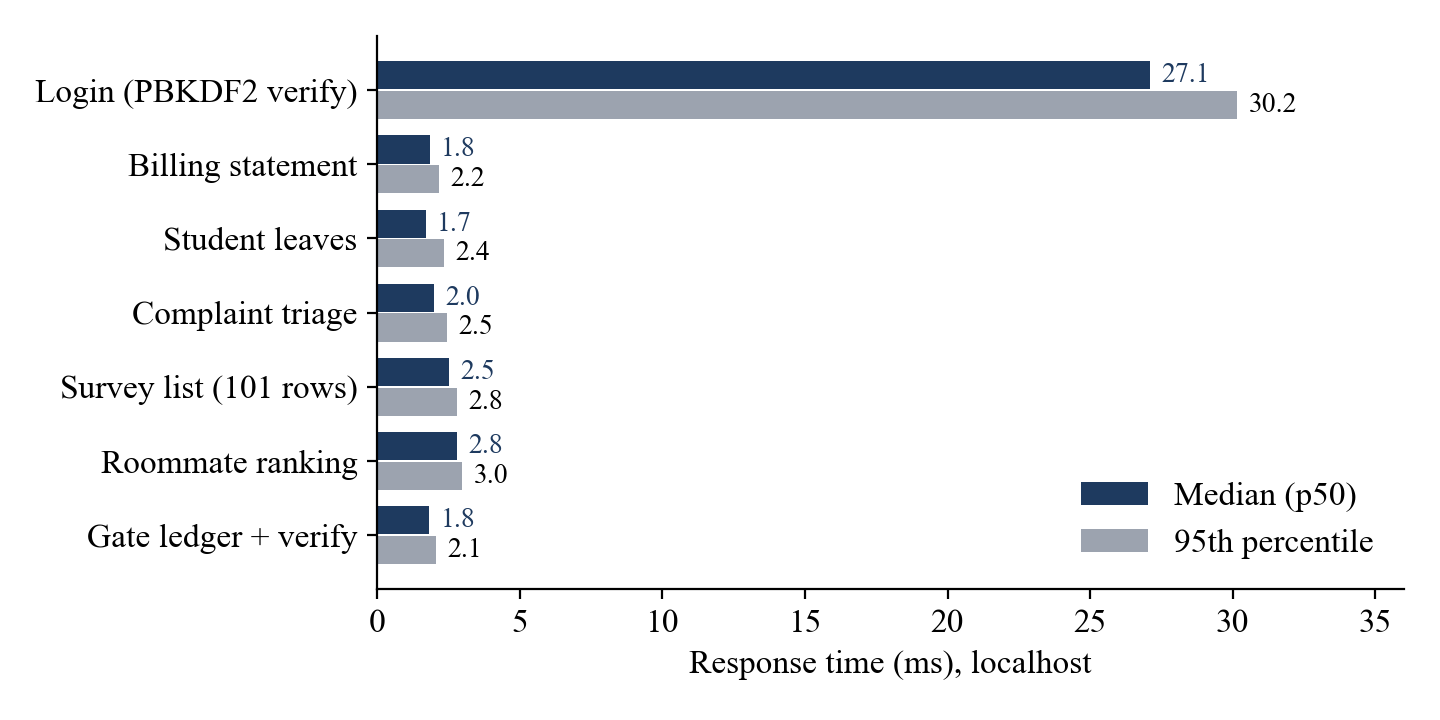
\includegraphics[width=0.7\linewidth]{latency.png}
\caption{Median and 95th-percentile response times of the seven core endpoints}\label{fig:latency}
\end{figure}

\section{Handbook assistant}
The first evaluation used 18 questions over six rulebooks: the correct rulebook was retrieved first for all 18, and
17 answers contained the expected fact. Extending the evaluation to every flow in the application exposed two
defects. The assistant's own suggested questions about visitor passes and leaves longer than three days had no
source text, so the model correctly declined to answer; two rulebooks describing the implemented workflows
(\texttt{visitors.md} and \texttt{leave.md}) were added. Second, the title line of each rulebook was indexed as a
separate chunk with no policy text and often outranked the real sections, which caused the earlier miss on the
laundry detergent question. Sections are now indexed with their rulebook title and title-only fragments are skipped,
and a weakly related second rulebook is no longer passed to the model.

The revised evaluation has 24 questions, three or more per rulebook across all eight. The correct rulebook was cited
first for \textbf{24 of 24} questions and every answer was correct on manual review (Table~\ref{tab:rag}); an
automatic substring check matched 22, the two misses being correct answers written with typographic hyphens and
non-breaking spaces. The median end-to-end answer time, including the Groq API call, was 0.70~s (maximum 4.8~s).

\begin{table}[!htbp]\centering\small
\caption{Handbook assistant evaluation (24 questions, eight rulebooks)}\label{tab:rag}
\begin{tabular}{p{3.0in}l}
\toprule\head \textbf{Metric} & \textbf{Result}\\\midrule
Correct rulebook cited first & 24/24 (100\%)\\
Answer correct (manual review) & 24/24 (100\%)\\
Expected fact matched automatically & 22/24 (91.7\%)\\
Median / maximum answer time (with LLM) & 0.70 s / 4.8 s\\
Index & 30 chunks from 8 rulebooks; about 31 s cold start\\
First evaluation (18 questions, 6 rulebooks) & 18/18 retrieved; 17/18 answered\\
\bottomrule
\end{tabular}
\end{table}

\section{Roommate compatibility on the 100-student dataset}
For each of the 100 seeded students, the other 99 were ranked with the student's own answers as the query. The 100
students have 56 distinct lifestyle profiles. Across all 9,900 ordered pairs the mean score is 53.9, but the best match
per student averages 96.7 with a minimum of 85, so every student has at least one highly compatible candidate
(Fig.~\ref{fig:compatdist}).

The analysis also exposed a real defect. Before the block constraint was added, the best match was of the same gender
for only 45 of 100 students, because the score ignores gender while Blocks A and B are single-gender. After restricting
candidates to the target block, Block A matches were same-gender for 44 of 44 students and Block B for 37 of 37. Block C
is mixed by design. The mean best-match score changed only from 97.0 to 96.7.

\begin{figure}[!htbp]\centering
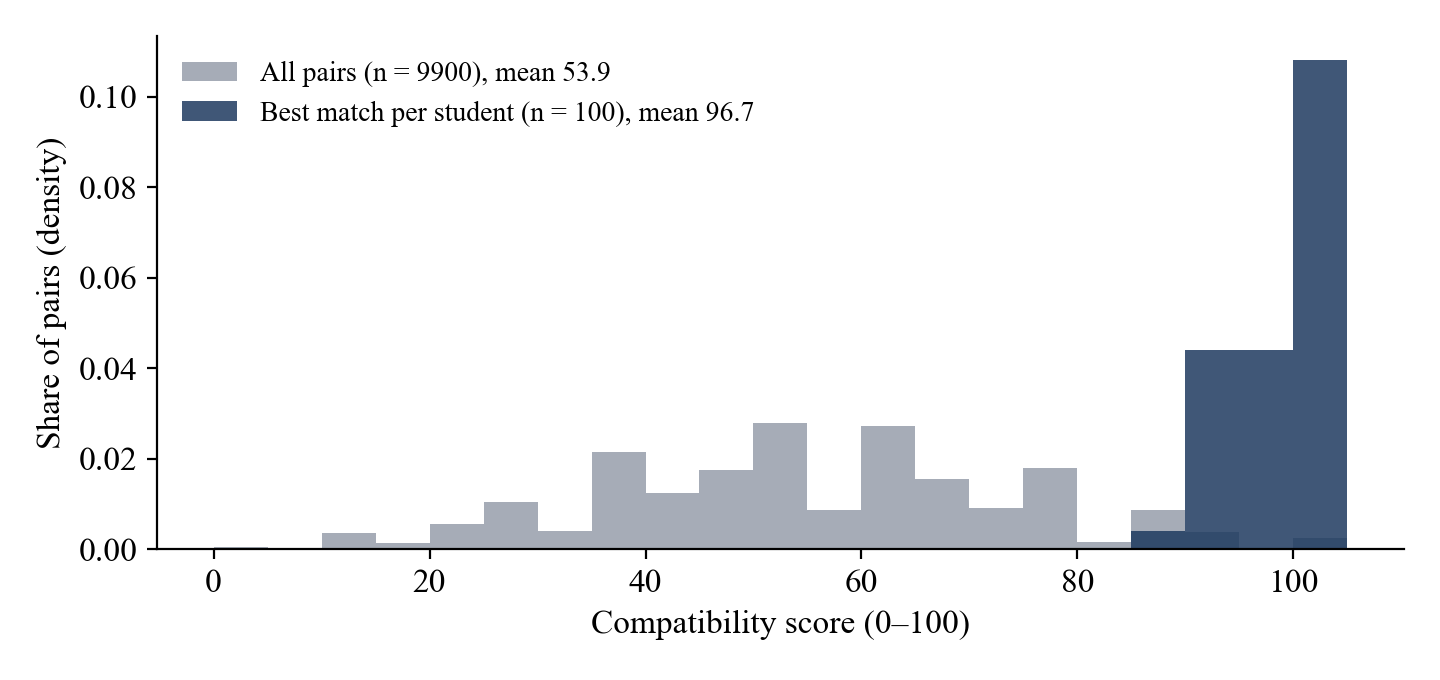
\includegraphics[width=0.7\linewidth]{compat.png}
\caption{Distribution of compatibility scores: all pairs versus each student's best match}\label{fig:compatdist}
\end{figure}

\section{Complaint triage}
A labelled sample of 30 realistic complaints (six per category: Electrical, Plumbing, IT/WiFi, Structural and General)
was used. The first version of the rules, which matched keywords anywhere inside words, classified 28 of 30 correctly
(93.3\%). Both errors were substring false positives: ``WiFi keeps disconnecting in Block A'' was labelled Structural
because ``Block'' contains ``lock'', and ``Need an extra blanket for winter'' was labelled IT / WiFi because
``blanket'' contains ``lan''. In addition, ``switch board gives a shock'' was not escalated as critical. Matching was
changed to word-start matching and ``shock'' was added as a hazard term. The revised rules classify 30 of 30 correctly
and flag both hazards as critical (Fig.~\ref{fig:quality}, left). Because the same sample guided the fix, this result is
optimistic, and a larger held-out set of real campus complaints is needed for an unbiased estimate
(Section~\ref{sec:limits}).

\section{Engineering quality}
Table~\ref{tab:quality} compares the hackathon prototype with this release. Route-level code splitting cut the
JavaScript downloaded on first visit by 81\% (Fig.~\ref{fig:quality}, right): modules such as the Excel parser and the
charting library load only on the screens that use them.

\begin{table}[!htbp]\centering\small
\caption{Prototype versus production release}\label{tab:quality}
\begin{tabularx}{\linewidth}{P{2.15in}P{1.6in}L}
\toprule\head \textbf{Measure} & \textbf{Prototype} & \textbf{This release}\\\midrule
Server-side authentication and authorisation & None (PINs checked in the browser) & Hashed credentials, signed sessions, role checks on every route\\
Data persistence & In memory, lost on restart & SQLite or DynamoDB, durable\\
ESLint errors & 65 & 0\\
High-severity production dependency advisories & 1 (xlsx 0.18.5) & 0\\
Automated tests & 0 & 41 (plus 57 browser checks)\\
Resident personal data at rest & Plain text & AES-256-GCM per field\\
On-screen text below 12 px & 70\% of text elements & None\\
First-load JavaScript (raw / gzip) & 1,316 kB / 386 kB & 254 kB / 76 kB\\
Deployment artefacts & None & Dockerfile, Compose file, CI workflow, health check\\
\bottomrule
\end{tabularx}
\end{table}

\begin{figure}[!htbp]\centering
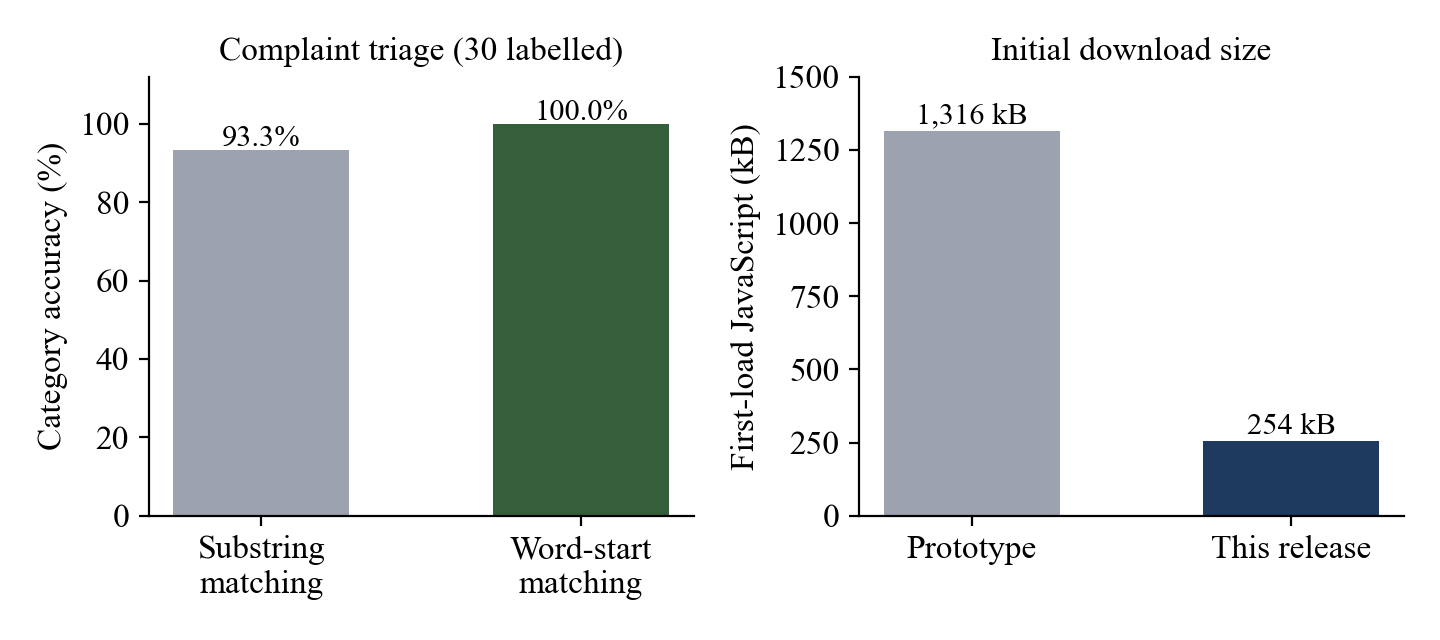
\includegraphics[width=0.72\linewidth]{quality.png}
\caption{Triage accuracy before and after the matching fix (left); first-load download size (right)}\label{fig:quality}
\end{figure}

\section{Readability audit}
Users reported that much of the interface text was hard to read. A script therefore measured every visible text
element on 33 screens (all modules for all four roles, plus the landing, persona and sign-in screens): its rendered
font size, and its contrast ratio against the background actually behind it, following WCAG 2.1 [30]. Most labels
used Courier New, a thin monospace face, at 8 to 11~px. The fix replaced it with IBM Plex Mono, raised every text size
to at least 12~px, lightened grey text on the dark footers, removed opacity dimming from resolved items and darkened
light status colours. Table~\ref{tab:readability} compares the two audits; the two remaining contrast flags are a
deliberately pulsing status indicator and a disabled button.

\begin{table}[!htbp]\centering\small
\caption{Readability audit before and after the redesign}\label{tab:readability}
\begin{tabular}{p{3.0in}cc}
\toprule\head \textbf{Measure} & \textbf{Before} & \textbf{After}\\\midrule
Text elements measured (33 screens) & 5,204 & 5,258\\
Text smaller than 12 px & 3,628 (70\%) & 0\\
Elements below WCAG contrast & 133 & 2\\
Smallest text size & 8 px & 12 px\\
Monospace typeface & Courier New & IBM Plex Mono\\
\bottomrule
\end{tabular}
\end{table}

\section{Discussion}
The results show that a modest stack with no GPU and a single small server is enough for the platform's workloads: data
endpoints respond in milliseconds and the assistant answers in well under two seconds. The evaluation also proved
valuable as a debugging tool: measuring the matching engine on the 100-student dataset revealed the cross-gender
recommendation problem, and the labelled triage sample revealed substring false positives. Both were fixed and are now covered by automated tests. Extending the assistant evaluation to every
workflow similarly revealed missing handbook coverage and a chunking flaw, and measuring the interface revealed that
most of its text was below a comfortable reading size. One inconsistency remains to be resolved with the administration: the room rulebook
promises a four-hour response for critical electrical or water faults, while the triage engine targets two hours, which
is stricter than the published policy.

% ================================================================== 6
\chapter{CONCLUSION AND FUTURE WORK}
\section{Summary}
Demeure AI turns a hackathon prototype into a deployable campus operating system. It unifies leave and visitor
approvals, room allocation, complaints, mess planning, grievances, facilities, billing and payment for four personas on
one persisted record, including 100 resident records whose personal details are encrypted at rest. Staff can
register residents individually or from a spreadsheet, with automatic bed assignment and hashed one-time access codes. Security is enforced on the server through hashed credentials, signed sessions, role and
ownership checks, validated input and private file storage. The hybrid design runs on a single machine or on AWS
DynamoDB, S3, SES and Polly without code changes. The intelligent features measured well: the handbook assistant
cited the right rulebook and answered correctly for all 24 evaluation questions; roommate matching gives every
student a best match scoring at least 85 while respecting single-gender blocks; and complaint triage classified all 30
labelled complaints after the word-matching fix. Fourteen end-to-end scenarios (57 browser checks) and 41 automated tests pass,
core API calls complete within 6~ms, and all on-screen text is at least 12~px.

\section{Limitations and Constraints}\label{sec:limits}
\begin{itemize}
  \item \textbf{Payments are simulated.} The UPI flow records a payment and receipt but is not connected to a payment
  gateway.
  \item \textbf{Simulated data sources.} Power telemetry, biometric gate scans and academic records (timetable, grades,
  library) are sample data; no meters, scanners or student information system are connected.
  \item \textbf{Small evaluation sets.} Triage was evaluated on 30 hand-written complaints that also guided the fix, and
  the assistant on 24 questions; larger held-out sets of real campus data are needed.
  \item \textbf{Rule-based triage.} Keyword rules are transparent but cannot understand paraphrases that use none of
  the keywords; the 2-hour critical target is stricter than the rulebook's 4-hour commitment.
  \item \textbf{Single-node local mode.} The SQLite store suits one server; multi-server deployments need the DynamoDB
  mode.
  \item \textbf{Deployment validation.} The container image and live AWS mode were not exercised on a cloud account
  during this evaluation, which ran in local mode.
  \item \textbf{Third-party AI.} Answer quality and latency depend on the external LLM provider, and the assistant
  returns raw policy text if the provider is unavailable.
  \item \textbf{Key management.} The encryption key is held in the server environment; there is no key
  rotation or hardware-backed key store yet, and losing the key makes encrypted fields unreadable.
\end{itemize}

\section{Improvement / Future Work}
\begin{itemize}
  \item Integrate a UPI payment gateway such as Razorpay or PayU with signed webhooks for reconciliation.
  \item Connect real data sources: smart energy meters for per-room billing, biometric gate hardware posting to the
  ledger API, and the university's student information system for academics.
  \item Replace keyword triage with a fine-tuned or embedding-based classifier trained on real tickets, keeping the
  rules as an explainable fallback.
  \item Add campus single sign-on (Google Workspace or Microsoft Entra ID) and multi-factor authentication for staff.
  \item Envelope encryption with AWS KMS, with scheduled key rotation and re-encryption of stored records.
  \item Section-level retrieval with re-ranking to fix misses such as the laundry detergent question.
  \item Constraint-aware stable roommate matching [19] for bulk allocation at the start of each semester.
  \item Push notifications and a mobile app; Hindi and regional-language interfaces for wider accessibility.
\end{itemize}

% ================================================================== 7
\chapter{SOCIAL AND ENVIRONMENTAL IMPACT}
\textbf{Student safety and well-being.} Anonymous anti-ragging reporting implements the confidential channel expected by
the UGC regulations [22] while keeping each case accountable through tracked status. Welfare alerts help wardens notice
residents who may need support, and hazardous complaints such as sparking sockets are escalated automatically.

\textbf{Transparency and trust.} Every approval is a recorded state change, students can track their own requests, and
the hash-chained gate ledger makes tampering with security records detectable. This supports accountable institutions
(SDG 16.6).

\textbf{Paperless operations.} Leave, visitor, booking and complaint forms that were previously printed and signed
become digital records, which reduces paper use and the time students spend queuing at offices.

\textbf{Energy and food.} Per-zone power monitoring and usage-based billing make consumption visible to administrators
and students (SDG 7.3). Published menus, meal ratings and wastage fines give mess managers the feedback needed to cut
food waste (SDG 12.3) [24].

\textbf{Low-cost, low-footprint deployment.} The whole platform runs on one small CPU-only server, and the AI component
uses a compact embedding model, so the system can be adopted by institutions with limited budgets.

\textbf{Privacy and ethics.} The system collects only operational data. Residents' contact, guardian, health and address details are
encrypted at rest and staff see masked numbers by default, in line with the safeguards expected under the DPDP Act
[27]. Uploaded documents are private to the student and authorised staff, anonymous grievances never expose the filer to staff, and the welfare module states that no
personal devices or audio are monitored. Wardens remain responsible for every decision; the compatibility and triage
outputs are recommendations, not automated decisions.

\textbf{Accessibility.} All on-screen text is at least 12~px with contrast checked against WCAG 2.1 [30], keyboard
focus is always visible, custom dropdowns and rating controls expose ARIA roles and labels for screen readers, and
assistant answers can be read aloud.

% ================================================================== 8
\chapter{WORK PLAN}
\section{Timeline}
The project ran from June to October 2026 in the phases shown in Table~\ref{tab:timeline}.
\begin{table}[!htbp]\centering\small
\caption{Project timeline (2026)}\label{tab:timeline}
\begin{tabularx}{\linewidth}{P{1.3in}P{1.75in}L}
\toprule\head \textbf{Period} & \textbf{Phase} & \textbf{Key outputs}\\\midrule
Early June & Problem study and design & Requirements, Figma wireframes for nine modules, 100-student survey dataset\\
13--14 June & WebForge hackathon prototype & React modules, FastAPI back end, RAG assistant over hostel rulebooks\\
July -- August & AWS integration & DynamoDB, S3, SES and Polly adapters; AWS Console Hub; hybrid mock mode\\
September & Feature expansion & Academic, facilities and finance hubs; documentation\\
October (weeks 1--2) & Production hardening & Server-side auth, persistence for all modules, validation, missing workflows\\
October (weeks 2--3) & Testing and evaluation & 32 tests, 10 end-to-end scenarios, latency and accuracy measurements\\
October (week 3) & Resident records and readability & Encrypted 100-resident database, onboarding and import, readability audit\\
October (week 4) & Deployment and reporting & Docker image, CI pipeline, presentation and this report\\
\bottomrule
\end{tabularx}
\end{table}

\section{Individual Contribution}
Table~\ref{tab:contrib} lists each member's contribution.
\begin{table}[!htbp]\centering\small
\caption{Individual contribution}\label{tab:contrib}
\begin{tabularx}{\linewidth}{P{1.6in}P{1.0in}L}
\toprule\head \textbf{Member} & \textbf{Register No.} & \textbf{Contribution}\\\midrule
Pratik Kumar & 24BML0027 & Project lead; system architecture; FastAPI back end, authentication and access control; AWS integration; RAG assistant\\
Thakur Chand Choudhary & 24BML0012 & Front-end modules (student services, security console, complaint desk, mess planner); UI testing and end-to-end scenarios\\
Nikunj Goydani & 24BEC0338 & Survey dataset and roommate compatibility; complaint triage evaluation; deployment (Docker, CI); documentation and report\\
\bottomrule
\end{tabularx}
\end{table}

% ================================================================== 9
\chapter{COST ANALYSIS}
\textbf{Development cost.} All software used is open source or free for development (Table~\ref{tab:sw}), and
development used the team's existing laptops, so the development cost was nil apart from internet access. In local mode
the platform needs no paid services.

\textbf{Operating cost.} Table~\ref{tab:cost} estimates the monthly cost of running Demeure AI on AWS for a hostel of
about 1,000 students. The workload assumptions are 2 million reads and 0.3 million writes per month, 10 GB of stored
documents, 20,000 notification e-mails, 2 million characters of speech synthesis and 30,000 assistant questions. Prices
are indicative on-demand list prices for the Mumbai (ap-south-1) region at the time of writing, converted at \inr85 per
US dollar; they should be confirmed with the AWS Pricing Calculator before procurement.

\begin{table}[!htbp]\centering\small
\caption{Indicative monthly operating cost on AWS (1,000 students)}\label{tab:cost}
\begin{tabularx}{\linewidth}{P{2.05in}L>{\centering\arraybackslash}p{0.8in}>{\centering\arraybackslash}p{0.85in}}
\toprule\head \textbf{Item} & \textbf{Basis} & \textbf{USD / month} & \textbf{INR / month}\\\midrule
Compute: EC2 t3.small + 20 GB gp3 disk & 730 hours, on demand & 18.20 & 1,547\\
Amazon DynamoDB (on-demand) & 2 M reads, 0.3 M writes, $<$ 1 GB stored & 1.30 & 111\\
Amazon S3 (private documents) & 10 GB Standard storage + requests & 0.30 & 26\\
Amazon SES (e-mail) & 20,000 e-mails at \$0.10 per 1,000 & 2.00 & 170\\
Amazon Polly (standard voices) & 2 M characters at \$4 per million & 8.00 & 680\\
LLM API for the assistant & 30,000 questions, $\sim$1,400 tokens each & $\approx$ 7.00 & $\approx$ 595\\
Domain and DNS (Route 53) & Hosted zone; TLS certificate free (ACM) & 0.60 & 51\\\midrule
\textbf{Total} & & \textbf{$\approx$ 37.40} & \textbf{$\approx$ 3,180}\\
\bottomrule
\end{tabularx}
\end{table}

This is about \inr3.2 per student per month, or roughly \inr38 per student per year. Running in local mode on an
existing campus server removes every line except the LLM API, and the assistant can fall back to returning retrieved
policy text at no cost. AWS Free Tier allowances further reduce the cost for the first year.

% ================================================================== 10
\chapter{REFERENCES}
\newcounter{refc}
\begin{list}{[\arabic{refc}]}{\usecounter{refc}\setlength{\labelwidth}{2.2em}\setlength{\leftmargin}{2.8em}%
  \setlength{\labelsep}{0.6em}\setlength{\itemsep}{4pt}\setlength{\parsep}{0pt}}
\setstretch{1.15}
\item P. Lewis, E. Perez, A. Piktus, F. Petroni, V. Karpukhin, N. Goyal, H. Küttler, M. Lewis, W. Yih, T. Rocktäschel, S. Riedel and D. Kiela, ``Retrieval-augmented generation for knowledge-intensive NLP tasks,'' in \emph{Proc. Advances in Neural Information Processing Systems (NeurIPS)}, vol.~33, 2020, pp.~9459--9474.
\item N. Reimers and I. Gurevych, ``Sentence-BERT: Sentence embeddings using Siamese BERT-networks,'' in \emph{Proc. Conf. Empirical Methods in Natural Language Processing (EMNLP-IJCNLP)}, 2019, pp.~3982--3992.
\item W. Wang, F. Wei, L. Dong, H. Bao, N. Yang and M. Zhou, ``MiniLM: Deep self-attention distillation for task-agnostic compression of pre-trained transformers,'' in \emph{Proc. Advances in Neural Information Processing Systems (NeurIPS)}, vol.~33, 2020, pp.~5776--5788.
\item A. Vaswani, N. Shazeer, N. Parmar, J. Uszkoreit, L. Jones, A. N. Gomez, Ł. Kaiser and I. Polosukhin, ``Attention is all you need,'' in \emph{Proc. Advances in Neural Information Processing Systems (NIPS)}, vol.~30, 2017, pp.~5998--6008.
\item F. T. Liu, K. M. Ting and Z.-H. Zhou, ``Isolation forest,'' in \emph{Proc. 8th IEEE Int. Conf. Data Mining (ICDM)}, 2008, pp.~413--422.
\item S. Haber and W. S. Stornetta, ``How to time-stamp a digital document,'' \emph{Journal of Cryptology}, vol.~3, no.~2, pp.~99--111, 1991.
\item S. Nakamoto, ``Bitcoin: A peer-to-peer electronic cash system,'' 2008. [Online]. Available: \url{https://bitcoin.org/bitcoin.pdf}
\item National Institute of Standards and Technology, ``Secure Hash Standard (SHS),'' FIPS PUB 180-4, Aug. 2015.
\item H. Krawczyk, M. Bellare and R. Canetti, ``HMAC: Keyed-hashing for message authentication,'' IETF RFC 2104, Feb. 1997.
\item K. Moriarty, B. Kaliski and A. Rusch, ``PKCS \#5: Password-based cryptography specification version 2.1,'' IETF RFC 8018, Jan. 2017.
\item A. Barth, ``HTTP state management mechanism,'' IETF RFC 6265, Apr. 2011.
\item P. A. Grassi, J. L. Fenton, E. M. Newton \emph{et al.}, ``Digital identity guidelines: Authentication and lifecycle management,'' NIST Special Publication 800-63B, Jun. 2017.
\item OWASP Foundation, ``OWASP Top 10:2021,'' 2021. [Online]. Available: \url{https://owasp.org/Top10/}
\item M. West, ``Content Security Policy Level 3,'' W3C Working Draft, World Wide Web Consortium. [Online]. Available: \url{https://www.w3.org/TR/CSP3/}
\item G. DeCandia, D. Hastorun, M. Jampani, G. Kakulapati, A. Lakshman, A. Pilchin, S. Sivasubramanian, P. Vosshall and W. Vogels, ``Dynamo: Amazon's highly available key-value store,'' in \emph{Proc. 21st ACM Symp. Operating Systems Principles (SOSP)}, 2007, pp.~205--220.
\item R. T. Fielding, ``Architectural styles and the design of network-based software architectures,'' Ph.D. dissertation, Univ. of California, Irvine, 2000.
\item Amazon Web Services, ``AWS Well-Architected Framework,'' AWS Whitepaper, 2023. [Online]. Available: \url{https://docs.aws.amazon.com/wellarchitected/latest/framework/}
\item D. Gale and L. S. Shapley, ``College admissions and the stability of marriage,'' \emph{The American Mathematical Monthly}, vol.~69, no.~1, pp.~9--15, 1962.
\item R. W. Irving, ``An efficient algorithm for the `stable roommates' problem,'' \emph{Journal of Algorithms}, vol.~6, no.~4, pp.~577--595, 1985.
\item Z. Min-Allah and S. Alrashed, ``Smart campus---A sketch,'' \emph{Sustainable Cities and Society}, vol.~59, Art. no.~102231, 2020.
\item A. Zanella, N. Bui, A. Castellani, L. Vangelista and M. Zorzi, ``Internet of Things for smart cities,'' \emph{IEEE Internet of Things Journal}, vol.~1, no.~1, pp.~22--32, Feb. 2014.
\item University Grants Commission, ``UGC Regulations on Curbing the Menace of Ragging in Higher Educational Institutions, 2009,'' New Delhi, India, 2009.
\item United Nations General Assembly, ``Transforming our world: The 2030 Agenda for Sustainable Development,'' Resolution A/RES/70/1, 2015.
\item United Nations Environment Programme, ``Food Waste Index Report 2021,'' Nairobi, Kenya, 2021.
\item OpenAI, ``gpt-oss-120b \& gpt-oss-20b model card,'' Aug. 2025. [Online]. Available: \url{https://openai.com/index/gpt-oss-model-card/}
\item Amazon Web Services, ``Amazon DynamoDB Developer Guide,'' ``Amazon S3 User Guide,'' ``Amazon SES Developer Guide'' and ``Amazon Polly Developer Guide,'' AWS Documentation. [Online]. Available: \url{https://docs.aws.amazon.com/}
\item Ministry of Electronics and Information Technology, Government of India, ``The Digital Personal Data Protection Act, 2023,'' Act No.~22 of 2023, Aug. 2023.
\item M. Dworkin, ``Recommendation for block cipher modes of operation: Galois/Counter Mode (GCM) and GMAC,'' NIST Special Publication 800-38D, Nov. 2007.
\item H. Krawczyk and P. Eronen, ``HMAC-based extract-and-expand key derivation function (HKDF),'' IETF RFC 5869, May 2010.
\item World Wide Web Consortium, ``Web Content Accessibility Guidelines (WCAG) 2.1,'' W3C Recommendation, Jun. 2018. [Online]. Available: \url{https://www.w3.org/TR/WCAG21/}
\end{list}

% ================================================================== 11
\chapter{APPENDIX-1: SOURCE CODE}
The complete source code (React front end, FastAPI back end, tests, Dockerfile and CI workflow) is in the project
repository. This appendix reproduces the core algorithms of Section~\ref{sec:algo}, including the field-level
encryption and bed assignment added for resident records.

\subsection*{A.1 Business rules: triage, compatibility and ledger (\texttt{backend/services/domain.py})}
\lstinputlisting{code/code_domain.py}
\subsection*{A.2 Signed session tokens (\texttt{backend/services/auth.py}, excerpt)}
\lstinputlisting{code/code_auth.py}
\subsection*{A.3 Role guard dependency (\texttt{backend/deps.py}, excerpt)}
\lstinputlisting{code/code_deps.py}
\subsection*{A.4 Field-level encryption (\texttt{backend/services/crypto.py}, excerpt)}
\lstinputlisting{code/code_crypto.py}
\subsection*{A.5 Bed assignment rules (\texttt{backend/services/rooms.py}, excerpt)}
\lstinputlisting{code/code_rooms.py}

\end{document}
